% Options for packages loaded elsewhere
\PassOptionsToPackage{unicode}{hyperref}
\PassOptionsToPackage{hyphens}{url}
%
\documentclass[
]{article}
\usepackage{amsmath,amssymb}
\usepackage{lmodern}
\usepackage{ifxetex,ifluatex}
\ifnum 0\ifxetex 1\fi\ifluatex 1\fi=0 % if pdftex
  \usepackage[T1]{fontenc}
  \usepackage[utf8]{inputenc}
  \usepackage{textcomp} % provide euro and other symbols
\else % if luatex or xetex
  \usepackage{unicode-math}
  \defaultfontfeatures{Scale=MatchLowercase}
  \defaultfontfeatures[\rmfamily]{Ligatures=TeX,Scale=1}
\fi
% Use upquote if available, for straight quotes in verbatim environments
\IfFileExists{upquote.sty}{\usepackage{upquote}}{}
\IfFileExists{microtype.sty}{% use microtype if available
  \usepackage[]{microtype}
  \UseMicrotypeSet[protrusion]{basicmath} % disable protrusion for tt fonts
}{}
\makeatletter
\@ifundefined{KOMAClassName}{% if non-KOMA class
  \IfFileExists{parskip.sty}{%
    \usepackage{parskip}
  }{% else
    \setlength{\parindent}{0pt}
    \setlength{\parskip}{6pt plus 2pt minus 1pt}}
}{% if KOMA class
  \KOMAoptions{parskip=half}}
\makeatother
\usepackage{xcolor}
\IfFileExists{xurl.sty}{\usepackage{xurl}}{} % add URL line breaks if available
\IfFileExists{bookmark.sty}{\usepackage{bookmark}}{\usepackage{hyperref}}
\hypersetup{
  hidelinks,
  pdfcreator={LaTeX via pandoc}}
\urlstyle{same} % disable monospaced font for URLs
\usepackage[margin=1in]{geometry}
\usepackage{color}
\usepackage{fancyvrb}
\newcommand{\VerbBar}{|}
\newcommand{\VERB}{\Verb[commandchars=\\\{\}]}
\DefineVerbatimEnvironment{Highlighting}{Verbatim}{commandchars=\\\{\}}
% Add ',fontsize=\small' for more characters per line
\usepackage{framed}
\definecolor{shadecolor}{RGB}{248,248,248}
\newenvironment{Shaded}{\begin{snugshade}}{\end{snugshade}}
\newcommand{\AlertTok}[1]{\textcolor[rgb]{0.94,0.16,0.16}{#1}}
\newcommand{\AnnotationTok}[1]{\textcolor[rgb]{0.56,0.35,0.01}{\textbf{\textit{#1}}}}
\newcommand{\AttributeTok}[1]{\textcolor[rgb]{0.77,0.63,0.00}{#1}}
\newcommand{\BaseNTok}[1]{\textcolor[rgb]{0.00,0.00,0.81}{#1}}
\newcommand{\BuiltInTok}[1]{#1}
\newcommand{\CharTok}[1]{\textcolor[rgb]{0.31,0.60,0.02}{#1}}
\newcommand{\CommentTok}[1]{\textcolor[rgb]{0.56,0.35,0.01}{\textit{#1}}}
\newcommand{\CommentVarTok}[1]{\textcolor[rgb]{0.56,0.35,0.01}{\textbf{\textit{#1}}}}
\newcommand{\ConstantTok}[1]{\textcolor[rgb]{0.00,0.00,0.00}{#1}}
\newcommand{\ControlFlowTok}[1]{\textcolor[rgb]{0.13,0.29,0.53}{\textbf{#1}}}
\newcommand{\DataTypeTok}[1]{\textcolor[rgb]{0.13,0.29,0.53}{#1}}
\newcommand{\DecValTok}[1]{\textcolor[rgb]{0.00,0.00,0.81}{#1}}
\newcommand{\DocumentationTok}[1]{\textcolor[rgb]{0.56,0.35,0.01}{\textbf{\textit{#1}}}}
\newcommand{\ErrorTok}[1]{\textcolor[rgb]{0.64,0.00,0.00}{\textbf{#1}}}
\newcommand{\ExtensionTok}[1]{#1}
\newcommand{\FloatTok}[1]{\textcolor[rgb]{0.00,0.00,0.81}{#1}}
\newcommand{\FunctionTok}[1]{\textcolor[rgb]{0.00,0.00,0.00}{#1}}
\newcommand{\ImportTok}[1]{#1}
\newcommand{\InformationTok}[1]{\textcolor[rgb]{0.56,0.35,0.01}{\textbf{\textit{#1}}}}
\newcommand{\KeywordTok}[1]{\textcolor[rgb]{0.13,0.29,0.53}{\textbf{#1}}}
\newcommand{\NormalTok}[1]{#1}
\newcommand{\OperatorTok}[1]{\textcolor[rgb]{0.81,0.36,0.00}{\textbf{#1}}}
\newcommand{\OtherTok}[1]{\textcolor[rgb]{0.56,0.35,0.01}{#1}}
\newcommand{\PreprocessorTok}[1]{\textcolor[rgb]{0.56,0.35,0.01}{\textit{#1}}}
\newcommand{\RegionMarkerTok}[1]{#1}
\newcommand{\SpecialCharTok}[1]{\textcolor[rgb]{0.00,0.00,0.00}{#1}}
\newcommand{\SpecialStringTok}[1]{\textcolor[rgb]{0.31,0.60,0.02}{#1}}
\newcommand{\StringTok}[1]{\textcolor[rgb]{0.31,0.60,0.02}{#1}}
\newcommand{\VariableTok}[1]{\textcolor[rgb]{0.00,0.00,0.00}{#1}}
\newcommand{\VerbatimStringTok}[1]{\textcolor[rgb]{0.31,0.60,0.02}{#1}}
\newcommand{\WarningTok}[1]{\textcolor[rgb]{0.56,0.35,0.01}{\textbf{\textit{#1}}}}
\usepackage{longtable,booktabs,array}
\usepackage{calc} % for calculating minipage widths
% Correct order of tables after \paragraph or \subparagraph
\usepackage{etoolbox}
\makeatletter
\patchcmd\longtable{\par}{\if@noskipsec\mbox{}\fi\par}{}{}
\makeatother
% Allow footnotes in longtable head/foot
\IfFileExists{footnotehyper.sty}{\usepackage{footnotehyper}}{\usepackage{footnote}}
\makesavenoteenv{longtable}
\usepackage{graphicx}
\makeatletter
\def\maxwidth{\ifdim\Gin@nat@width>\linewidth\linewidth\else\Gin@nat@width\fi}
\def\maxheight{\ifdim\Gin@nat@height>\textheight\textheight\else\Gin@nat@height\fi}
\makeatother
% Scale images if necessary, so that they will not overflow the page
% margins by default, and it is still possible to overwrite the defaults
% using explicit options in \includegraphics[width, height, ...]{}
\setkeys{Gin}{width=\maxwidth,height=\maxheight,keepaspectratio}
% Set default figure placement to htbp
\makeatletter
\def\fps@figure{htbp}
\makeatother
\setlength{\emergencystretch}{3em} % prevent overfull lines
\providecommand{\tightlist}{%
  \setlength{\itemsep}{0pt}\setlength{\parskip}{0pt}}
\setcounter{secnumdepth}{5}
\usepackage{booktabs}
\ifluatex
  \usepackage{selnolig}  % disable illegal ligatures
\fi
\usepackage[]{natbib}
\bibliographystyle{plainnat}

\author{}
\date{\vspace{-2.5em}}

\begin{document}

{
\setcounter{tocdepth}{2}
\tableofcontents
}
\hypertarget{uxc815uxaddcuxc131-uxac80uxc815normality-test}{%
\section{정규성 검정(Normality Test)}\label{uxc815uxaddcuxc131-uxac80uxc815normality-test}}

\hypertarget{uxb370uxc774uxd130-uxbd88uxb7ecuxc624uxae30}{%
\subsection{데이터 불러오기}\label{uxb370uxc774uxd130-uxbd88uxb7ecuxc624uxae30}}

\begin{Shaded}
\begin{Highlighting}[]
\NormalTok{my.data }\OtherTok{\textless{}{-}}\NormalTok{ ToothGrowth}
\FunctionTok{str}\NormalTok{(my.data)}
\end{Highlighting}
\end{Shaded}

\begin{verbatim}
## 'data.frame':    60 obs. of  3 variables:
##  $ len : num  4.2 11.5 7.3 5.8 6.4 10 11.2 11.2 5.2 7 ...
##  $ supp: Factor w/ 2 levels "OJ","VC": 2 2 2 2 2 2 2 2 2 2 ...
##  $ dose: num  0.5 0.5 0.5 0.5 0.5 0.5 0.5 0.5 0.5 0.5 ...
\end{verbatim}

R에 있는 기본 데이터셋인 ToothGrowth를 불러온다.
3개의 변수와 60개의 관측치가 있다.

\hypertarget{uxc815uxaddcuxc131-uxac80uxc815uxc774uxb780}{%
\subsection{정규성 검정이란}\label{uxc815uxaddcuxc131-uxac80uxc815uxc774uxb780}}

데이터셋의 분포가 정규분포를 따르는지 검정하는 것을 말한다.

데이터셋이 정규분포를 따라야, 다양한 분석 이론을 적용시킬 수 있다.

만일, 정규분포를 따르지 않는다면 데이터 먼징하거나 비모수적 방법을 사용한다.

\hypertarget{uxc911uxc694uxd55c-uxb450-uxbc95uxce59}{%
\subsection{중요한 두 법칙}\label{uxc911uxc694uxd55c-uxb450-uxbc95uxce59}}

다음 두 법칙으로 인해, 대표본(n\textgreater=30)인 경우 데이터셋은 정규분포를 따른다.

\textbf{중심극한의 정리(C.L.T - Central Limit Theorem)}

\begin{itemize}
\item
  표본의 평균은 표본의 크기가 커질수록, 정규분표와 유사해진다.
\item
  모집단이 정규분포하지 않더라도 표본의 크기가 충분히 크다면, 정규분포라고 가정할 수 있다.
\end{itemize}

\textbf{대수의 법칙}

\begin{itemize}
\item
  표본의 크기가 증가할수록, 통계적 추정의 정밀도가 향상된다는 것을 수학적으로 증명
\item
  표본의 크기가 커짐에 따라 표본에서 계산한 평균값과 모집단의 실제평균과의 차이가 매우 작아진다.
\end{itemize}

\textbf{정규성 검정 시각화}

\begin{itemize}
\tightlist
\item
  ggdensity
\end{itemize}

\begin{Shaded}
\begin{Highlighting}[]
\FunctionTok{library}\NormalTok{(ggpubr)}
\end{Highlighting}
\end{Shaded}

\begin{verbatim}
## Loading required package: ggplot2
\end{verbatim}

\begin{Shaded}
\begin{Highlighting}[]
\FunctionTok{ggdensity}\NormalTok{(my.data}\SpecialCharTok{$}\NormalTok{len,}
          \AttributeTok{add =} \StringTok{"mean"}\NormalTok{,}
          \AttributeTok{color =} \StringTok{"red"}\NormalTok{,}
          \AttributeTok{fill =} \StringTok{"violet red"}\NormalTok{,}
          \AttributeTok{alpha =}\NormalTok{ .}\DecValTok{5}\NormalTok{,}
          \AttributeTok{title =} \StringTok{"Dendity plot of Tooth Length"}\NormalTok{,}
          \AttributeTok{xlab =} \StringTok{"Tooth Length"}\NormalTok{)}
\end{Highlighting}
\end{Shaded}

\begin{verbatim}
## Warning: geom_vline(): Ignoring `mapping` because `xintercept` was provided.
\end{verbatim}

\begin{verbatim}
## Warning: geom_vline(): Ignoring `data` because `xintercept` was provided.
\end{verbatim}

\includegraphics{NormalityTest_files/figure-latex/unnamed-chunk-2-1.pdf}

\begin{itemize}
\tightlist
\item
  ggqqplot
\end{itemize}

\begin{Shaded}
\begin{Highlighting}[]
\FunctionTok{library}\NormalTok{(ggpubr)}
\FunctionTok{ggqqplot}\NormalTok{(my.data}\SpecialCharTok{$}\NormalTok{len, }\AttributeTok{color =} \StringTok{"red"}\NormalTok{)}
\end{Highlighting}
\end{Shaded}

\includegraphics{NormalityTest_files/figure-latex/unnamed-chunk-3-1.pdf}

\begin{itemize}
\tightlist
\item
  qqPlot
\end{itemize}

\begin{Shaded}
\begin{Highlighting}[]
\FunctionTok{library}\NormalTok{(car)}
\end{Highlighting}
\end{Shaded}

\begin{verbatim}
## Loading required package: carData
\end{verbatim}

\begin{Shaded}
\begin{Highlighting}[]
\FunctionTok{qqPlot}\NormalTok{(my.data}\SpecialCharTok{$}\NormalTok{len)}
\end{Highlighting}
\end{Shaded}

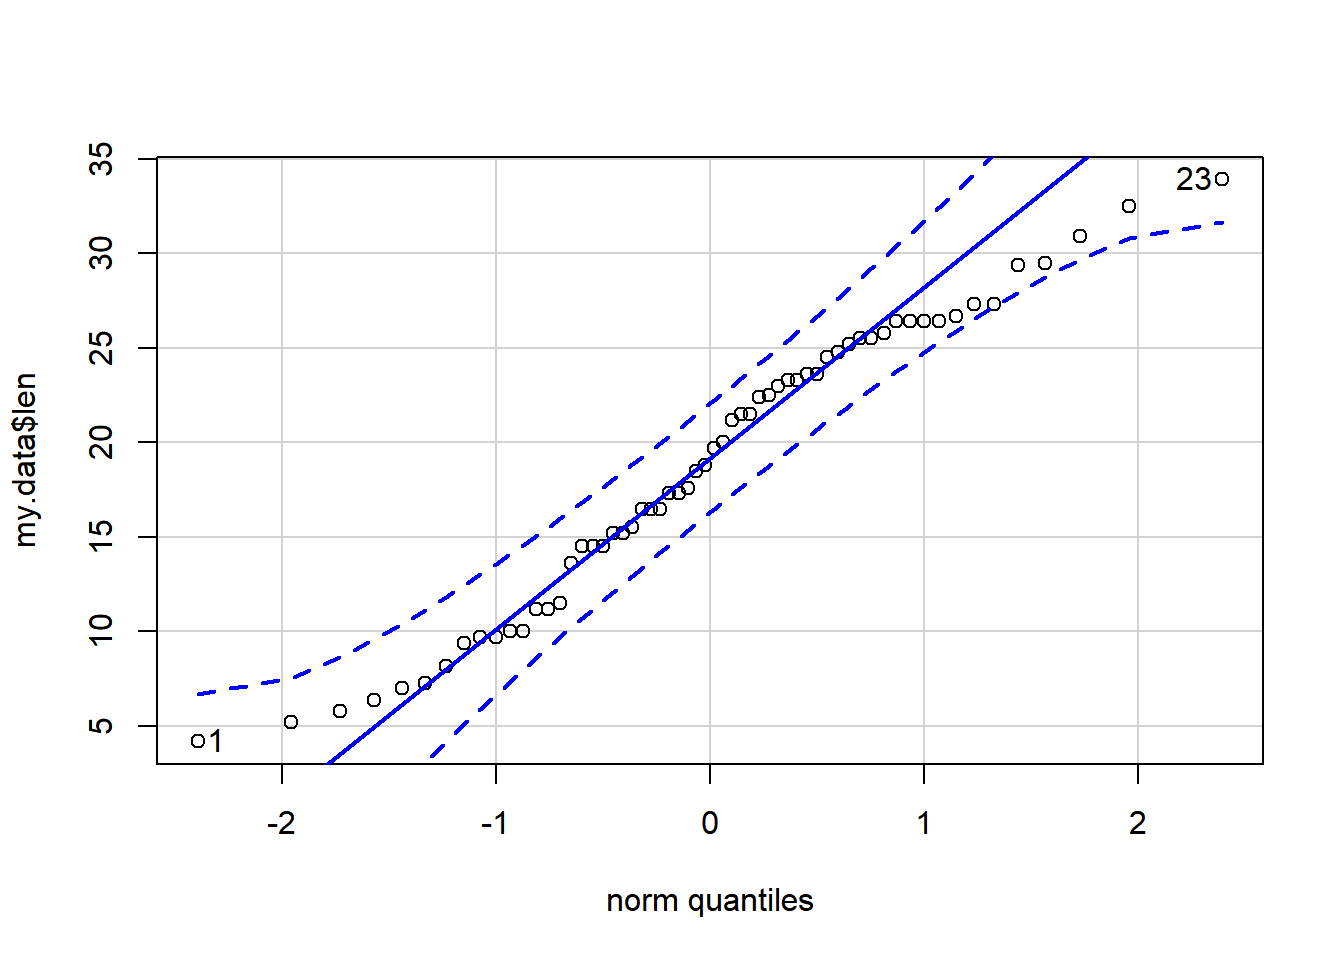
\includegraphics{NormalityTest_files/figure-latex/unnamed-chunk-4-1.pdf}

\begin{verbatim}
## [1] 23  1
\end{verbatim}

\begin{itemize}
\tightlist
\item
  따로 그리기
\end{itemize}

\begin{Shaded}
\begin{Highlighting}[]
\FunctionTok{qqnorm}\NormalTok{(my.data}\SpecialCharTok{$}\NormalTok{len)}
\FunctionTok{qqline}\NormalTok{(my.data}\SpecialCharTok{$}\NormalTok{len, }\AttributeTok{col =}\DecValTok{2}\NormalTok{)}
\end{Highlighting}
\end{Shaded}

\includegraphics{NormalityTest_files/figure-latex/unnamed-chunk-5-1.pdf}

\hypertarget{shapiro-wilk-uxac80uxc815}{%
\subsection{Shapiro-Wilk 검정}\label{shapiro-wilk-uxac80uxc815}}

귀무가설 H0 : 모집단은 \textbf{정규분포를 따른다}.
대립가설 H1 : 모집단은 \textbf{정규분포를 따르지 않는다}.

\begin{Shaded}
\begin{Highlighting}[]
\FunctionTok{shapiro.test}\NormalTok{(my.data}\SpecialCharTok{$}\NormalTok{len)}
\end{Highlighting}
\end{Shaded}

\begin{verbatim}
## 
##  Shapiro-Wilk normality test
## 
## data:  my.data$len
## W = 0.96743, p-value = 0.1091
\end{verbatim}

\begin{Shaded}
\begin{Highlighting}[]
\DocumentationTok{\#\# }
\DocumentationTok{\#\#  Shapiro{-}Wilk normality test}
\DocumentationTok{\#\# }
\DocumentationTok{\#\# data:  my.data$len}
\DocumentationTok{\#\# W = 0.96743, p{-}value = 0.1091}
\end{Highlighting}
\end{Shaded}

p값이 0.05보다 크기 때문에
귀무가설 채택한다.
정규성을 따른다.

\hypertarget{uxb4f1uxbd84uxc0b0uxc131-uxac80uxc815homogeneity-of-variance-test}{%
\section{등분산성 검정(Homogeneity of Variance Test)}\label{uxb4f1uxbd84uxc0b0uxc131-uxac80uxc815homogeneity-of-variance-test}}

\hypertarget{uxb370uxc774uxd130-uxbd88uxb7ecuxc624uxae30-1}{%
\subsection{데이터 불러오기}\label{uxb370uxc774uxd130-uxbd88uxb7ecuxc624uxae30-1}}

\begin{Shaded}
\begin{Highlighting}[]
\FunctionTok{data}\NormalTok{(ToothGrowth)}
\FunctionTok{data}\NormalTok{(PlantGrowth)}
\FunctionTok{str}\NormalTok{(ToothGrowth)}
\end{Highlighting}
\end{Shaded}

\begin{verbatim}
## 'data.frame':    60 obs. of  3 variables:
##  $ len : num  4.2 11.5 7.3 5.8 6.4 10 11.2 11.2 5.2 7 ...
##  $ supp: Factor w/ 2 levels "OJ","VC": 2 2 2 2 2 2 2 2 2 2 ...
##  $ dose: num  0.5 0.5 0.5 0.5 0.5 0.5 0.5 0.5 0.5 0.5 ...
\end{verbatim}

\begin{Shaded}
\begin{Highlighting}[]
\FunctionTok{str}\NormalTok{(PlantGrowth)}
\end{Highlighting}
\end{Shaded}

\begin{verbatim}
## 'data.frame':    30 obs. of  2 variables:
##  $ weight: num  4.17 5.58 5.18 6.11 4.5 4.61 5.17 4.53 5.33 5.14 ...
##  $ group : Factor w/ 3 levels "ctrl","trt1",..: 1 1 1 1 1 1 1 1 1 1 ...
\end{verbatim}

R에 있는 기본 데이터셋인 ToothGrowth를 불러온다.

3개의 변수와 60개의 관측치가 있다.

\hypertarget{uxb4f1uxbd84uxc0b0uxc131-uxac80uxc815uxc774uxb780}{%
\subsection{등분산성 검정이란}\label{uxb4f1uxbd84uxc0b0uxc131-uxac80uxc815uxc774uxb780}}

\begin{itemize}
\item
  등분산성인지 아닌지를 구분하는 방법이다.
\item
  등분산성은 분산분석할때 기본적으로 만족해야되는 조건 중 한가지로, 분석하는 집단들의 분산이 같음을 의미한다.
\item
  검정의 방법은 두 집단, 다 집단일때 달라진다. 또한 모수, 비모수에 따라 달라진다.
\end{itemize}

\hypertarget{uxb450-uxc9d1uxb2e8uxc77cuxb54c}{%
\subsection{두 집단일때}\label{uxb450-uxc9d1uxb2e8uxc77cuxb54c}}

\hypertarget{f-test}{%
\subsubsection{F test}\label{f-test}}

반드시 정규성이 있어야 한다.

귀무가설 H0 : 등분산성이 있다(분산의 차이가 없다).

대립가설 H1 : 등분산성이 없다(분산의 차이가 있다).

\begin{Shaded}
\begin{Highlighting}[]
\NormalTok{res.ftest }\OtherTok{\textless{}{-}} \FunctionTok{var.test}\NormalTok{(len }\SpecialCharTok{\textasciitilde{}}\NormalTok{ supp, }\AttributeTok{data =}\NormalTok{ ToothGrowth, }\AttributeTok{alternative =} \StringTok{"two.sided"}\NormalTok{)}
\NormalTok{res.ftest}
\end{Highlighting}
\end{Shaded}

\begin{verbatim}
## 
##  F test to compare two variances
## 
## data:  len by supp
## F = 0.6386, num df = 29, denom df = 29, p-value = 0.2331
## alternative hypothesis: true ratio of variances is not equal to 1
## 95 percent confidence interval:
##  0.3039488 1.3416857
## sample estimates:
## ratio of variances 
##          0.6385951
\end{verbatim}

두 변수 len과 supp의 등분산성을 검정했을때,

p-value 값이 유의수준(0.05)보다 큰 0.2331로 나왔다.

따라서 귀무가설을 채택하여 등분산성이 있다.

여기서 , alternative는 양측 검정할지 단측 검정할지를 설정해준다.

\begin{Shaded}
\begin{Highlighting}[]
\NormalTok{res.ftest}\SpecialCharTok{$}\NormalTok{estimate}
\end{Highlighting}
\end{Shaded}

\begin{verbatim}
## ratio of variances 
##          0.6385951
\end{verbatim}

등분산 검정 함수에는 분산이 얼마나 같은지 알려주는 estimate가 있다.
여기서는 약 63.8\% 분산이 같다.

\hypertarget{uxb2e4uxc9d1uxb2e8-uxc77cuxb54c}{%
\subsection{다집단 일때}\label{uxb2e4uxc9d1uxb2e8-uxc77cuxb54c}}

\hypertarget{bartletts-test}{%
\subsubsection{Bartlett's test}\label{bartletts-test}}

\begin{itemize}
\item
  반드시 정규성이 있어야 한다.
\item
  귀무가설 H0 : 등분산성이 있다(분산의 차이가 없다).
\item
  대립가설 H1 : 등분산성이 없다(분산의 차이가 있다).
\end{itemize}

\begin{Shaded}
\begin{Highlighting}[]
\FunctionTok{bartlett.test}\NormalTok{(weight }\SpecialCharTok{\textasciitilde{}}\NormalTok{ group, }\AttributeTok{data =}\NormalTok{ PlantGrowth)}
\end{Highlighting}
\end{Shaded}

\begin{verbatim}
## 
##  Bartlett test of homogeneity of variances
## 
## data:  weight by group
## Bartlett's K-squared = 2.8786, df = 2, p-value = 0.2371
\end{verbatim}

PlantGrowth의 group 변수에는 세 가지 요인이 있기 때문에 다 집단이다.

그리고 p-value 값이 유의수준(0.05)보다 큰 0.2371로 나왔다.

따라서 귀무가설을 채택하여 등분산성이 있다.

\hypertarget{levenes-test}{%
\subsubsection{Levene's test}\label{levenes-test}}

\{car\} 패키지에 있다.

정규성이 있어야 하는 전제 조건에 덜 민감하다.

귀무가설 H0 : 등분산성이 있다(분산의 차이가 없다).

대립가설 H1 : 등분산성이 없다(분산의 차이가 있다).

\begin{Shaded}
\begin{Highlighting}[]
\FunctionTok{library}\NormalTok{(car)}
\end{Highlighting}
\end{Shaded}

\begin{verbatim}
## Loading required package: carData
\end{verbatim}

\begin{Shaded}
\begin{Highlighting}[]
\FunctionTok{leveneTest}\NormalTok{(weight }\SpecialCharTok{\textasciitilde{}}\NormalTok{ group, }\AttributeTok{data =}\NormalTok{ PlantGrowth)}
\end{Highlighting}
\end{Shaded}

\begin{verbatim}
## Levene's Test for Homogeneity of Variance (center = median)
##       Df F value Pr(>F)
## group  2  1.1192 0.3412
##       27
\end{verbatim}

p-value 값이 유의수준(0.05)보다 큰 0.3412로 나왔다.

따라서 귀무가설을 채택하여 등분산성이 있다.

\hypertarget{fligner-killeen-test}{%
\subsubsection{Fligner-Killeen test}\label{fligner-killeen-test}}

비모수적 방법이다.

따라서 표본의 크기, 확률 분포와 상관이 없다.

귀무가설 H0 : 등분산성이 있다(분산의 차이가 없다).

대립가설 H1 : 등분산성이 없다(분산의 차이가 있다).

\begin{Shaded}
\begin{Highlighting}[]
\FunctionTok{fligner.test}\NormalTok{(weight }\SpecialCharTok{\textasciitilde{}}\NormalTok{ group, }\AttributeTok{data =}\NormalTok{ PlantGrowth)}
\end{Highlighting}
\end{Shaded}

\begin{verbatim}
## 
##  Fligner-Killeen test of homogeneity of variances
## 
## data:  weight by group
## Fligner-Killeen:med chi-squared = 2.3499, df = 2, p-value = 0.3088
\end{verbatim}

PlantGrowth는 표본이 충분히 커서 모수적 방법을 쓰지만, 여기서 연습용으로 다룬다.

p-value 값이 유의수준(0.05)보다 큰 0.3088로 나왔다.

따라서 귀무가설을 채택하여 등분산성이 있다.

\hypertarget{uxb3c5uxb9bduxc131-uxac80uxc815test-of-independence}{%
\section{독립성 검정(Test of Independence)}\label{uxb3c5uxb9bduxc131-uxac80uxc815test-of-independence}}

\hypertarget{uxb370uxc774uxd130-uxbd88uxb7ecuxc624uxae30-2}{%
\subsection{데이터 불러오기}\label{uxb370uxc774uxd130-uxbd88uxb7ecuxc624uxae30-2}}

\begin{Shaded}
\begin{Highlighting}[]
\FunctionTok{library}\NormalTok{(ggplot2)}
\FunctionTok{data}\NormalTok{(mpg)}
\NormalTok{mpg }\OtherTok{\textless{}{-}} \FunctionTok{as.data.frame}\NormalTok{(mpg)}
\FunctionTok{str}\NormalTok{(mpg)}
\end{Highlighting}
\end{Shaded}

\begin{verbatim}
## 'data.frame':    234 obs. of  11 variables:
##  $ manufacturer: chr  "audi" "audi" "audi" "audi" ...
##  $ model       : chr  "a4" "a4" "a4" "a4" ...
##  $ displ       : num  1.8 1.8 2 2 2.8 2.8 3.1 1.8 1.8 2 ...
##  $ year        : int  1999 1999 2008 2008 1999 1999 2008 1999 1999 2008 ...
##  $ cyl         : int  4 4 4 4 6 6 6 4 4 4 ...
##  $ trans       : chr  "auto(l5)" "manual(m5)" "manual(m6)" "auto(av)" ...
##  $ drv         : chr  "f" "f" "f" "f" ...
##  $ cty         : int  18 21 20 21 16 18 18 18 16 20 ...
##  $ hwy         : int  29 29 31 30 26 26 27 26 25 28 ...
##  $ fl          : chr  "p" "p" "p" "p" ...
##  $ class       : chr  "compact" "compact" "compact" "compact" ...
\end{verbatim}

ggplot2 패키지에 있는 mpg를 불러온다.

11개의 변수와 234개의 관측치가 있다.

\hypertarget{uxad50uxcc28uxd45ccross-tabulation-uxc0dduxc131}{%
\subsection{교차표(cross tabulation) 생성}\label{uxad50uxcc28uxd45ccross-tabulation-uxc0dduxc131}}

\begin{Shaded}
\begin{Highlighting}[]
\FunctionTok{library}\NormalTok{(prettyR)}
\NormalTok{(crosstab}\OtherTok{\textless{}{-}}\FunctionTok{xtabs}\NormalTok{(}\AttributeTok{formula =} \SpecialCharTok{\textasciitilde{}}\NormalTok{fl}\SpecialCharTok{+}\NormalTok{drv, }\AttributeTok{data =}\NormalTok{ mpg))}
\end{Highlighting}
\end{Shaded}

\begin{verbatim}
##    drv
## fl   4  f  r
##   c  0  1  0
##   d  2  3  0
##   e  6  1  1
##   p 20 25  7
##   r 75 76 17
\end{verbatim}

fl(연료타입)과 drv(구동방식)의 교차표를 만들어 살펴본다.

데이터셋의 분포를 알고, 상황에 맞는 함수를 사용한다.

\hypertarget{uxb3c5uxb9bduxc131-uxac80uxc815uxc774uxb780}{%
\subsection{독립성 검정이란}\label{uxb3c5uxb9bduxc131-uxac80uxc815uxc774uxb780}}

두 변수가 독립적인지, 즉 관계가 있는지를 알려주는 통계기법이다.

변수가 범주형인 경우 카이제곱 검정을 사용하고,

연속형인 경우 공분산을 사용한다.

\hypertarget{uxbc94uxc8fcuxd615-uxbcc0uxc218uxac04uxc5d0-uxac80uxc815}{%
\subsection{범주형 변수간에 검정}\label{uxbc94uxc8fcuxd615-uxbcc0uxc218uxac04uxc5d0-uxac80uxc815}}

\hypertarget{uxce74uxc774uxc81cuxacf1-uxac80uxc815uxc774uxb780}{%
\subsubsection{카이제곱 검정이란}\label{uxce74uxc774uxc81cuxacf1-uxac80uxc815uxc774uxb780}}

카이제곱 분포에 기초한 통계적 방법으로, 관찰된 빈도가 기대되는 빈도와 의미있게 다른지의 여부를 검증하기 위해 사용되는 검증방법이다.

*자료가 빈도로 주어졌을 때, 특히 명목척도 자료의 분석에 이용된다.

*쉽게 말하면, 변수간의 차이가 있는지 없는지를 검정해준다. (변수간의 독립성을 검정해준다)

귀무가설(H0): A, B는 서로 차이가 없다 (관계가 없다, 독립이다)

대립가설(H1): A, B는 서로 차이가 있다 (관계가 있다, 독립이 아니다)
Pearson's Chi-squared Test(피어슨의 카이제곱 검정)

표본의 크기가 큰 경우에 사용한다.

\begin{Shaded}
\begin{Highlighting}[]
\FunctionTok{chisq.test}\NormalTok{(crosstab, }\AttributeTok{correct =} \ConstantTok{TRUE}\NormalTok{)}
\end{Highlighting}
\end{Shaded}

\begin{verbatim}
## Warning in chisq.test(crosstab, correct = TRUE): Chi-squared approximation may
## be incorrect
\end{verbatim}

\begin{verbatim}
## 
##  Pearson's Chi-squared test
## 
## data:  crosstab
## X-squared = 6.5618, df = 8, p-value = 0.5846
\end{verbatim}

p-value 값이 유의수준(0.05)보다 크기 때문에 귀무가설 채택.

따라서, 연료타입과 구동방식은 관계가 없다.

\hypertarget{fishers-exact-testuxd53cuxc154uxc758-uxac80uxc815}{%
\subsubsection{Fisher's Exact Test(피셔의 검정)}\label{fishers-exact-testuxd53cuxc154uxc758-uxac80uxc815}}

\begin{itemize}
\tightlist
\item
  표본수가 적거나
\item
  표본의 교차표를 보았을때, 특정 셀에 매우 치우치게 분포되어 있을 경우
\end{itemize}

카이제곱 검정 이후, 피셔의 정확한 검정을 해야 한다.

앞서 살펴본 교차표에서 연료타입 p,r에 치우쳐 있다.
따라서 피셔의 정확한 검정을 한다.

\begin{Shaded}
\begin{Highlighting}[]
\FunctionTok{fisher.test}\NormalTok{(crosstab, }\AttributeTok{alternative =} \StringTok{\textquotesingle{}two.sided\textquotesingle{}}\NormalTok{)}
\end{Highlighting}
\end{Shaded}

\begin{verbatim}
## 
##  Fisher's Exact Test for Count Data
## 
## data:  crosstab
## p-value = 0.5121
## alternative hypothesis: two.sided
\end{verbatim}

정확한 검정을 적용해도 같은 결과가 나온다.

\hypertarget{uxc5f0uxc18duxd615-uxbcc0uxc218uxac04uxc5d0-uxac80uxc815}{%
\subsection{연속형 변수간에 검정}\label{uxc5f0uxc18duxd615-uxbcc0uxc218uxac04uxc5d0-uxac80uxc815}}

\hypertarget{uxacf5uxbd84uxc0b0covariance}{%
\subsubsection{공분산(covariance)}\label{uxacf5uxbd84uxc0b0covariance}}

공분산이란

\begin{itemize}
\tightlist
\item
  두 확률변수가 얼마나 함께 변화하는지 측정
\item
  양의 값이면 비례관계, 음의 값이면 반비례관계, 0이면 관계가 없다.
\end{itemize}

++ 한 변수가 커질 때, 다른 변수가 함께 커지거나 한 변수가 작아질 때, 다른 변수가 함께 작아지는 것과 같이, 크기변화의 방향이 같다면, 공분산은 양의값을 가짐

++ 한 변수가 커질 때, 다른 변수가 작아지거나 한 변수가 작아질 때, 다른 변수가 커지는 것과 같이, 크기변화의 방향이 다르다면, 공분산은 음의값을 가짐

++ 만약 두 변수의 값이 서로 상관없이 변한다면, 공분산은 0 임

\begin{Shaded}
\begin{Highlighting}[]
\FunctionTok{cov}\NormalTok{(mpg}\SpecialCharTok{$}\NormalTok{cty,mpg}\SpecialCharTok{$}\NormalTok{hwy)}
\end{Highlighting}
\end{Shaded}

\begin{verbatim}
## [1] 24.22543
\end{verbatim}

mpg 데이터셋에 있는 cty(도시연비)와 hwy(고속도로 연비)의 공분산 검정을 한다.

24.22로 양의 값이 나왔기 때문에 두 변수는 관계가 있다.

\hypertarget{one-sample-t-test}{%
\section{One Sample T-test}\label{one-sample-t-test}}

모집단에 대한 평균이 참인지를 알아보고 신뢰구간도 구할 수 있다.

\hypertarget{uxb370uxc774uxd130-uxb9ccuxb4e4uxae30}{%
\subsection{데이터 만들기}\label{uxb370uxc774uxd130-uxb9ccuxb4e4uxae30}}

\begin{Shaded}
\begin{Highlighting}[]
\FunctionTok{set.seed}\NormalTok{(}\DecValTok{1234}\NormalTok{)}
\NormalTok{my.data }\OtherTok{\textless{}{-}} \FunctionTok{data.frame}\NormalTok{( }\AttributeTok{name =} \FunctionTok{paste0}\NormalTok{( }\FunctionTok{rep}\NormalTok{(}\StringTok{"M\_"}\NormalTok{, }\DecValTok{10}\NormalTok{), }\DecValTok{1}\SpecialCharTok{:}\DecValTok{10}\NormalTok{ ), }\AttributeTok{weight =} \FunctionTok{round}\NormalTok{( }\FunctionTok{rnorm}\NormalTok{(}\DecValTok{40}\NormalTok{, }\DecValTok{90}\NormalTok{, }\DecValTok{2}\NormalTok{), }\DecValTok{1}\NormalTok{ ) )}

\FunctionTok{str}\NormalTok{(my.data)}
\end{Highlighting}
\end{Shaded}

\begin{verbatim}
## 'data.frame':    40 obs. of  2 variables:
##  $ name  : chr  "M_1" "M_2" "M_3" "M_4" ...
##  $ weight: num  87.6 90.6 92.2 85.3 90.9 91 88.9 88.9 88.9 88.2 ...
\end{verbatim}

남자 10명에 대한 이름과 몸무게를 담은 데이터셋을 만든다.

\hypertarget{one-sample-t-testuxb780}{%
\subsection{One sample T-test란}\label{one-sample-t-testuxb780}}

모집단에 대한 평균이 참인지를 알아보고 신뢰구간도 구할 수 있다.

예시)

귀무가설: 강남구에 사는 사람들의 평균 소득이 500만원이다.

대립가설: 강남구에 사는 사람들의 평균 소득이 500만원이 아니다.

\hypertarget{uxbaa8uxc218uxc801-uxbc29uxbc95}{%
\subsection{모수적 방법}\label{uxbaa8uxc218uxc801-uxbc29uxbc95}}

모수적인 방법을 사용하기 위해서는 모집단이 정규성을 따르는지 확인해야 한다.

앞에서 만든 데이터(my.data)가 소표본이기 때문이다.

\hypertarget{uxc815uxaddcuxc131-uxac80uxc815}{%
\subsection{정규성 검정}\label{uxc815uxaddcuxc131-uxac80uxc815}}

\begin{Shaded}
\begin{Highlighting}[]
\FunctionTok{shapiro.test}\NormalTok{(my.data}\SpecialCharTok{$}\NormalTok{weight)}
\end{Highlighting}
\end{Shaded}

\begin{verbatim}
## 
##  Shapiro-Wilk normality test
## 
## data:  my.data$weight
## W = 0.96003, p-value = 0.1679
\end{verbatim}

p-value값이 유의수준(0.05)보다 크기 때문에 귀무가설 채택.

따라서 정규성을 따른다.

\hypertarget{t.test}{%
\subsection{t.test}\label{t.test}}

\begin{Shaded}
\begin{Highlighting}[]
\FunctionTok{summary}\NormalTok{(my.data}\SpecialCharTok{$}\NormalTok{weight)}
\end{Highlighting}
\end{Shaded}

\begin{verbatim}
##    Min. 1st Qu.  Median    Mean 3rd Qu.    Max. 
##   85.30   88.17   89.00   89.17   90.15   94.80
\end{verbatim}

summary함수를 이용하면 남자 10명의 평균 몸무게가 89.17kg라는 것을 알 수 있다.

만약 평균 몸무게를 모른다고 가정하고 가설을 잡는다.

남자 평균 몸무게가 95kg이다.(귀무가설)

\begin{Shaded}
\begin{Highlighting}[]
\NormalTok{(res}\OtherTok{\textless{}{-}}\FunctionTok{t.test}\NormalTok{(my.data}\SpecialCharTok{$}\NormalTok{weight,}\AttributeTok{mu =} \DecValTok{95}\NormalTok{))}
\end{Highlighting}
\end{Shaded}

\begin{verbatim}
## 
##  One Sample t-test
## 
## data:  my.data$weight
## t = -20.175, df = 39, p-value < 2.2e-16
## alternative hypothesis: true mean is not equal to 95
## 95 percent confidence interval:
##  88.58551 89.75449
## sample estimates:
## mean of x 
##     89.17
\end{verbatim}

p-value값이 유의수준(0.05)보다 아주 작기 때문에 귀무가설 기각. 대립가설 채택.

따라서, 남자 평균 몸무게가 95kg이 아니다.

alternative를 사용하여 대립가설을 조정할 수 있다.

\begin{Shaded}
\begin{Highlighting}[]
\FunctionTok{t.test}\NormalTok{(my.data}\SpecialCharTok{$}\NormalTok{weight, }\AttributeTok{mu =} \DecValTok{95}\NormalTok{, }\AttributeTok{alternative =} \StringTok{"less"}\NormalTok{)}
\end{Highlighting}
\end{Shaded}

\begin{verbatim}
## 
##  One Sample t-test
## 
## data:  my.data$weight
## t = -20.175, df = 39, p-value < 2.2e-16
## alternative hypothesis: true mean is less than 95
## 95 percent confidence interval:
##      -Inf 89.65688
## sample estimates:
## mean of x 
##     89.17
\end{verbatim}

less인 경우, 남자 평균 몸무게가 95kg보다 작다.(대립가설) 대립가설 채택이기 때문에 대립가설이 참이다.

\begin{Shaded}
\begin{Highlighting}[]
\FunctionTok{t.test}\NormalTok{(my.data}\SpecialCharTok{$}\NormalTok{weight, }\AttributeTok{mu =} \DecValTok{95}\NormalTok{, }\AttributeTok{alternative =} \StringTok{"greater"}\NormalTok{)}
\end{Highlighting}
\end{Shaded}

\begin{verbatim}
## 
##  One Sample t-test
## 
## data:  my.data$weight
## t = -20.175, df = 39, p-value = 1
## alternative hypothesis: true mean is greater than 95
## 95 percent confidence interval:
##  88.68312      Inf
## sample estimates:
## mean of x 
##     89.17
\end{verbatim}

greater인 경우, 남자 평균 몸무게가 95kg보다 크다.(대립가설) 귀무가설 채택이기 때문에 대립가설이 거짓이다.

신뢰구간

\begin{Shaded}
\begin{Highlighting}[]
\NormalTok{res}\SpecialCharTok{$}\NormalTok{conf.int}
\end{Highlighting}
\end{Shaded}

\begin{verbatim}
## [1] 88.58551 89.75449
## attr(,"conf.level")
## [1] 0.95
\end{verbatim}

값이 88.58551\textasciitilde89.75449 사이가 신뢰구간 0.95이내 이다.

\hypertarget{uxbe44uxbaa8uxc218uxc801-uxbc29uxbc95}{%
\subsection{비모수적 방법}\label{uxbe44uxbaa8uxc218uxc801-uxbc29uxbc95}}

소표본이고 정규성을 따르지 않을 때 사용하는 방법이다.

\begin{Shaded}
\begin{Highlighting}[]
\FunctionTok{set.seed}\NormalTok{(}\DecValTok{1234}\NormalTok{)}
\NormalTok{my.data2 }\OtherTok{\textless{}{-}} \FunctionTok{data.frame}\NormalTok{( }\AttributeTok{name =} \FunctionTok{paste0}\NormalTok{( }\FunctionTok{rep}\NormalTok{(}\StringTok{"M\_"}\NormalTok{, }\DecValTok{10}\NormalTok{), }\DecValTok{1}\SpecialCharTok{:}\DecValTok{10}\NormalTok{ ), }\AttributeTok{weight =} \FunctionTok{round}\NormalTok{( }\FunctionTok{rnorm}\NormalTok{(}\DecValTok{70}\NormalTok{, }\DecValTok{90}\NormalTok{, }\DecValTok{2}\NormalTok{), }\DecValTok{1}\NormalTok{ ) )}

\FunctionTok{str}\NormalTok{(my.data2)}
\end{Highlighting}
\end{Shaded}

\begin{verbatim}
## 'data.frame':    70 obs. of  2 variables:
##  $ name  : chr  "M_1" "M_2" "M_3" "M_4" ...
##  $ weight: num  87.6 90.6 92.2 85.3 90.9 91 88.9 88.9 88.9 88.2 ...
\end{verbatim}

\begin{Shaded}
\begin{Highlighting}[]
\FunctionTok{shapiro.test}\NormalTok{(my.data2}\SpecialCharTok{$}\NormalTok{weight)}
\end{Highlighting}
\end{Shaded}

\begin{verbatim}
## 
##  Shapiro-Wilk normality test
## 
## data:  my.data2$weight
## W = 0.94492, p-value = 0.003967
\end{verbatim}

my.data는 정규성을 따르기 때문에 살짝 조정해 준다.

\hypertarget{wilcox.testuxc70cuxcf55uxc2a8-uxac80uxc815}{%
\subsubsection{wilcox.test(윌콕슨 검정)}\label{wilcox.testuxc70cuxcf55uxc2a8-uxac80uxc815}}

\begin{Shaded}
\begin{Highlighting}[]
\FunctionTok{wilcox.test}\NormalTok{(my.data2}\SpecialCharTok{$}\NormalTok{weight,}\AttributeTok{mu=}\DecValTok{95}\NormalTok{)}
\end{Highlighting}
\end{Shaded}

\begin{verbatim}
## 
##  Wilcoxon signed rank test with continuity correction
## 
## data:  my.data2$weight
## V = 1, p-value = 3.761e-13
## alternative hypothesis: true location is not equal to 95
\end{verbatim}

p-value값이 유의수준(0.05)보다 아주 작기 때문에 귀무가설 기각. 대립가설 채택.

따라서, 남자 평균 몸무게가 95kg이 아니다.

추가 옵션

\begin{Shaded}
\begin{Highlighting}[]
\FunctionTok{t.test}\NormalTok{(my.data2}\SpecialCharTok{$}\NormalTok{weight, }\AttributeTok{mu =} \DecValTok{95}\NormalTok{, }\AttributeTok{alternative =} \StringTok{"less"}\NormalTok{)}
\end{Highlighting}
\end{Shaded}

\begin{verbatim}
## 
##  One Sample t-test
## 
## data:  my.data2$weight
## t = -22.665, df = 69, p-value < 2.2e-16
## alternative hypothesis: true mean is less than 95
## 95 percent confidence interval:
##      -Inf 89.85957
## sample estimates:
## mean of x 
##  89.45143
\end{verbatim}

\begin{Shaded}
\begin{Highlighting}[]
\FunctionTok{t.test}\NormalTok{(my.data2}\SpecialCharTok{$}\NormalTok{weight, }\AttributeTok{mu =} \DecValTok{95}\NormalTok{, }\AttributeTok{alternative =} \StringTok{"greater"}\NormalTok{)}
\end{Highlighting}
\end{Shaded}

\begin{verbatim}
## 
##  One Sample t-test
## 
## data:  my.data2$weight
## t = -22.665, df = 69, p-value = 1
## alternative hypothesis: true mean is greater than 95
## 95 percent confidence interval:
##  89.04328      Inf
## sample estimates:
## mean of x 
##  89.45143
\end{verbatim}

모수적 방법과 똑같이 해석하면 된다.

\hypertarget{paired-samples-t-test}{%
\section{Paired samples T-test}\label{paired-samples-t-test}}

\hypertarget{uxb370uxc774uxd130-uxb9ccuxb4e4uxae30-1}{%
\subsection{데이터 만들기}\label{uxb370uxc774uxd130-uxb9ccuxb4e4uxae30-1}}

\begin{Shaded}
\begin{Highlighting}[]
\NormalTok{before }\OtherTok{\textless{}{-}}\FunctionTok{c}\NormalTok{(}\FloatTok{200.1}\NormalTok{, }\FloatTok{190.9}\NormalTok{, }\FloatTok{192.7}\NormalTok{, }\DecValTok{213}\NormalTok{, }\FloatTok{241.4}\NormalTok{, }\FloatTok{196.9}\NormalTok{, }\FloatTok{172.2}\NormalTok{, }\FloatTok{185.5}\NormalTok{, }\FloatTok{205.2}\NormalTok{, }\FloatTok{193.7}\NormalTok{)}
\NormalTok{after }\OtherTok{\textless{}{-}}\FunctionTok{c}\NormalTok{(}\FloatTok{392.9}\NormalTok{, }\FloatTok{393.2}\NormalTok{, }\FloatTok{345.1}\NormalTok{, }\DecValTok{393}\NormalTok{, }\DecValTok{434}\NormalTok{, }\FloatTok{427.9}\NormalTok{, }\DecValTok{422}\NormalTok{, }\FloatTok{383.9}\NormalTok{, }\FloatTok{392.3}\NormalTok{, }\FloatTok{352.2}\NormalTok{)    }

\NormalTok{( my.data }\OtherTok{\textless{}{-}} \FunctionTok{data.frame}\NormalTok{(}\AttributeTok{group =} \FunctionTok{rep}\NormalTok{(}\FunctionTok{c}\NormalTok{(}\StringTok{"before"}\NormalTok{, }\StringTok{"after"}\NormalTok{), }\AttributeTok{each =} \DecValTok{10}\NormalTok{), }\AttributeTok{weight =} \FunctionTok{c}\NormalTok{(before, after) ) )}
\end{Highlighting}
\end{Shaded}

\begin{verbatim}
##     group weight
## 1  before  200.1
## 2  before  190.9
## 3  before  192.7
## 4  before  213.0
## 5  before  241.4
## 6  before  196.9
## 7  before  172.2
## 8  before  185.5
## 9  before  205.2
## 10 before  193.7
## 11  after  392.9
## 12  after  393.2
## 13  after  345.1
## 14  after  393.0
## 15  after  434.0
## 16  after  427.9
## 17  after  422.0
## 18  after  383.9
## 19  after  392.3
## 20  after  352.2
\end{verbatim}

각각 10개씩 전(before), 후(after)에 대한 weight를 담은 데이터셋을 만든다.

\hypertarget{paired-samples-t-testuxb780}{%
\subsection{Paired samples T-test란}\label{paired-samples-t-testuxb780}}

대응표본(1:1 비교가능한 그룹or군)에 대한 평균차이가 있는지 검정하는 방법이다.

예시)

귀무가설: 강남구에 사는 사람의 2009년 소득은 2010년의 소득과 같다.

대립가설: 강남구에 사는 사람의 2009년 소득은 2010년의 소득과 다르다.

\hypertarget{uxc2dcuxac01uxd654uxb85c-uxd655uxc778uxd558uxae30}{%
\subsection{시각화로 확인하기}\label{uxc2dcuxac01uxd654uxb85c-uxd655uxc778uxd558uxae30}}

\begin{Shaded}
\begin{Highlighting}[]
\FunctionTok{library}\NormalTok{(}\StringTok{"ggpubr"}\NormalTok{)}
\end{Highlighting}
\end{Shaded}

\begin{verbatim}
## Loading required package: ggplot2
\end{verbatim}

\begin{Shaded}
\begin{Highlighting}[]
\FunctionTok{ggboxplot}\NormalTok{(my.data, }
          \AttributeTok{x =} \StringTok{"group"}\NormalTok{,}
          \AttributeTok{y =} \StringTok{"weight"}\NormalTok{, }
          \AttributeTok{color =} \StringTok{"group"}\NormalTok{,}
          \AttributeTok{palette =} \FunctionTok{c}\NormalTok{(}\StringTok{"\#00AFBB"}\NormalTok{, }\StringTok{"\#E7B800"}\NormalTok{),}
          \AttributeTok{order =} \FunctionTok{c}\NormalTok{(}\StringTok{"before"}\NormalTok{, }\StringTok{"after"}\NormalTok{),}
          \AttributeTok{ylab =} \StringTok{"Weight"}\NormalTok{,}
          \AttributeTok{xlab =} \StringTok{"Groups"}\NormalTok{)}
\end{Highlighting}
\end{Shaded}

\includegraphics{T-testPaired_files/figure-latex/unnamed-chunk-2-1.pdf}

before after 나누기

\begin{Shaded}
\begin{Highlighting}[]
\NormalTok{before }\OtherTok{\textless{}{-}} \FunctionTok{subset}\NormalTok{(my.data,  group }\SpecialCharTok{==} \StringTok{"before"}\NormalTok{, weight, }\AttributeTok{drop =} \ConstantTok{TRUE}\NormalTok{)}
\end{Highlighting}
\end{Shaded}

\begin{Shaded}
\begin{Highlighting}[]
\NormalTok{after }\OtherTok{\textless{}{-}} \FunctionTok{subset}\NormalTok{(my.data,  group }\SpecialCharTok{==} \StringTok{"after"}\NormalTok{, weight, }\AttributeTok{drop =} \ConstantTok{TRUE}\NormalTok{)}
\end{Highlighting}
\end{Shaded}

\hypertarget{uxd50cuxb86f-uxbe44uxad50-uxd568uxc218}{%
\subsubsection{플롯 비교 함수}\label{uxd50cuxb86f-uxbe44uxad50-uxd568uxc218}}

\begin{Shaded}
\begin{Highlighting}[]
\FunctionTok{library}\NormalTok{(PairedData)}
\end{Highlighting}
\end{Shaded}

\begin{verbatim}
## Loading required package: MASS
\end{verbatim}

\begin{verbatim}
## Loading required package: gld
\end{verbatim}

\begin{verbatim}
## Loading required package: mvtnorm
\end{verbatim}

\begin{verbatim}
## Loading required package: lattice
\end{verbatim}

\begin{verbatim}
## 
## Attaching package: 'PairedData'
\end{verbatim}

\begin{verbatim}
## The following object is masked from 'package:base':
## 
##     summary
\end{verbatim}

\begin{Shaded}
\begin{Highlighting}[]
\NormalTok{pd }\OtherTok{\textless{}{-}} \FunctionTok{paired}\NormalTok{(before, after)}
\FunctionTok{plot}\NormalTok{(pd, }\AttributeTok{type =} \StringTok{"profile"}\NormalTok{) }\SpecialCharTok{+} \FunctionTok{theme\_bw}\NormalTok{()}
\end{Highlighting}
\end{Shaded}

\includegraphics{T-testPaired_files/figure-latex/unnamed-chunk-5-1.pdf}

plot 함수로 봐도 충분히 차이가 있다는 것을 확인할 수 있다.

\hypertarget{uxbaa8uxc218uxc801-uxbc29uxbc95-1}{%
\subsection{모수적 방법}\label{uxbaa8uxc218uxc801-uxbc29uxbc95-1}}

모수적인 방법을 사용하기 위해서는 두 가지 전제 조건이 필요하다.

즉, 모집단이 정규성과 등분산성을 따르는지 확인해야 한다.
정규성 검정

\begin{Shaded}
\begin{Highlighting}[]
\FunctionTok{shapiro.test}\NormalTok{(my.data}\SpecialCharTok{$}\NormalTok{weight[my.data}\SpecialCharTok{$}\NormalTok{group}\SpecialCharTok{==}\StringTok{"before"}\NormalTok{])}
\end{Highlighting}
\end{Shaded}

\begin{verbatim}
## 
##  Shapiro-Wilk normality test
## 
## data:  my.data$weight[my.data$group == "before"]
## W = 0.90938, p-value = 0.2768
\end{verbatim}

\begin{Shaded}
\begin{Highlighting}[]
\FunctionTok{shapiro.test}\NormalTok{(my.data}\SpecialCharTok{$}\NormalTok{weight[my.data}\SpecialCharTok{$}\NormalTok{group}\SpecialCharTok{==}\StringTok{"after"}\NormalTok{])}
\end{Highlighting}
\end{Shaded}

\begin{verbatim}
## 
##  Shapiro-Wilk normality test
## 
## data:  my.data$weight[my.data$group == "after"]
## W = 0.91121, p-value = 0.2894
\end{verbatim}

둘 다 p-value값이 유의수준(0.05)보다 크기 때문에 귀무가설 채택.

따라서 정규성을 따른다.

\hypertarget{uxb4f1uxbd84uxc0b0uxc131-uxac80uxc815}{%
\subsection{등분산성 검정}\label{uxb4f1uxbd84uxc0b0uxc131-uxac80uxc815}}

\begin{Shaded}
\begin{Highlighting}[]
\FunctionTok{var.test}\NormalTok{(weight}\SpecialCharTok{\textasciitilde{}}\NormalTok{group, }\AttributeTok{data =}\NormalTok{ my.data)}
\end{Highlighting}
\end{Shaded}

\begin{verbatim}
## 
##  F test to compare two variances
## 
## data:  weight by group
## F = 2.5324, num df = 9, denom df = 9, p-value = 0.1825
## alternative hypothesis: true ratio of variances is not equal to 1
## 95 percent confidence interval:
##   0.6290172 10.1955065
## sample estimates:
## ratio of variances 
##            2.53242
\end{verbatim}

p-value값이 유의수준(0.05)보다 크기 때문에 귀무가설 채택.

따라서 등분산성을 따른다.

두 전제조건 모두 만족한다.

\hypertarget{t.test-1}{%
\subsection{t.test}\label{t.test-1}}

\begin{Shaded}
\begin{Highlighting}[]
\NormalTok{( res }\OtherTok{\textless{}{-}} \FunctionTok{t.test}\NormalTok{(weight }\SpecialCharTok{\textasciitilde{}}\NormalTok{ group, }\AttributeTok{data =}\NormalTok{ my.data, }\AttributeTok{paired =} \ConstantTok{TRUE}\NormalTok{) )}
\end{Highlighting}
\end{Shaded}

\begin{verbatim}
## 
##  Paired t-test
## 
## data:  weight by group
## t = 20.883, df = 9, p-value = 6.2e-09
## alternative hypothesis: true difference in means is not equal to 0
## 95 percent confidence interval:
##  173.4219 215.5581
## sample estimates:
## mean of the differences 
##                  194.49
\end{verbatim}

p-value값이 유의수준(0.05)보다 아주 작기 때문에 귀무가설 기각. 대립가설 채택.

따라서, before, after의 weight 차이가 있다.

추가 옵션

table(my.data\$group)

t.test(weight \textasciitilde{} group, data = my.data, paired = TRUE, alternative = ``less'')

t.test(weight \textasciitilde{} group, data = my.data, paired = TRUE, alternative = ``greater'')

alternative를 사용하여 대립가설을 조정할 수 있다.

여기서는 table함수를 통해 어떤 그룹이 먼저 들어갔는지 확인한다. after가 먼저다. 가설에서 순서가 정해지기 때문이다.

less인 경우, after의 weihgt가 before weihgt보다 작다.(대립가설) 귀무가설 채택이기 때문에 대립가설이 거짓이다.

greater인 경우, after의 weihgt가 before weihgt보다 크다.(대립가설) 대립가설 채택이기 때문에 대립가설이 참이다.

\hypertarget{uxd3c9uxade0-uxcd94uxc815-uxac12uxacfc-uxc2e0uxb8b0uxad6cuxac04}{%
\subsection{평균 추정 값과 신뢰구간}\label{uxd3c9uxade0-uxcd94uxc815-uxac12uxacfc-uxc2e0uxb8b0uxad6cuxac04}}

\begin{Shaded}
\begin{Highlighting}[]
\NormalTok{res}\SpecialCharTok{$}\NormalTok{estimate}
\end{Highlighting}
\end{Shaded}

\begin{verbatim}
## mean of the differences 
##                  194.49
\end{verbatim}

\begin{Shaded}
\begin{Highlighting}[]
\NormalTok{res}\SpecialCharTok{$}\NormalTok{conf.int}
\end{Highlighting}
\end{Shaded}

\begin{verbatim}
## [1] 173.4219 215.5581
## attr(,"conf.level")
## [1] 0.95
\end{verbatim}

after의 weihgt와 before weihgt의 차이 값은 194.49이다.

before, after의 weight 차이 값이 173.4219\textasciitilde215.5581 사이가 신뢰구간 0.95이내 이다.

\hypertarget{uxbe44uxbaa8uxc218uxc801-uxbc29uxbc95-1}{%
\subsection{비모수적 방법}\label{uxbe44uxbaa8uxc218uxc801-uxbc29uxbc95-1}}

소표본이고 정규성을 따르지 않을 때 사용하는 방법이다.

my.data는 전제조건을 통과하여 모수적 방법을 사용해야 하지만 연습으로 그냥 한다.
\#\#\# wilcox.test(윌콕슨 검정)

\begin{Shaded}
\begin{Highlighting}[]
\FunctionTok{wilcox.test}\NormalTok{(weight }\SpecialCharTok{\textasciitilde{}}\NormalTok{ group, }\AttributeTok{data =}\NormalTok{ my.data, }\AttributeTok{paired =} \ConstantTok{TRUE}\NormalTok{)}
\end{Highlighting}
\end{Shaded}

\begin{verbatim}
## 
##  Wilcoxon signed rank exact test
## 
## data:  weight by group
## V = 55, p-value = 0.001953
## alternative hypothesis: true location shift is not equal to 0
\end{verbatim}

p-value값이 유의수준(0.05)보다 작기 때문에 귀무가설 기각. 대립가설 채택.

따라서, before, after의 weight 차이가 있다.

\hypertarget{uxcd94uxac00-uxc635uxc158}{%
\subsection{추가 옵션}\label{uxcd94uxac00-uxc635uxc158}}

\begin{Shaded}
\begin{Highlighting}[]
\FunctionTok{table}\NormalTok{(my.data}\SpecialCharTok{$}\NormalTok{group)}
\end{Highlighting}
\end{Shaded}

\begin{verbatim}
## 
##  after before 
##     10     10
\end{verbatim}

\begin{Shaded}
\begin{Highlighting}[]
\FunctionTok{wilcox.test}\NormalTok{(weight }\SpecialCharTok{\textasciitilde{}}\NormalTok{ group, }\AttributeTok{data =}\NormalTok{ my.data, }\AttributeTok{paired =} \ConstantTok{TRUE}\NormalTok{, }\AttributeTok{alternative =} \StringTok{"less"}\NormalTok{)}
\end{Highlighting}
\end{Shaded}

\begin{verbatim}
## 
##  Wilcoxon signed rank exact test
## 
## data:  weight by group
## V = 55, p-value = 1
## alternative hypothesis: true location shift is less than 0
\end{verbatim}

\begin{Shaded}
\begin{Highlighting}[]
\FunctionTok{wilcox.test}\NormalTok{(weight }\SpecialCharTok{\textasciitilde{}}\NormalTok{ group, }\AttributeTok{data =}\NormalTok{ my.data, }\AttributeTok{paired =} \ConstantTok{TRUE}\NormalTok{, }\AttributeTok{alternative =} \StringTok{"greater"}\NormalTok{)}
\end{Highlighting}
\end{Shaded}

\begin{verbatim}
## 
##  Wilcoxon signed rank exact test
## 
## data:  weight by group
## V = 55, p-value = 0.0009766
## alternative hypothesis: true location shift is greater than 0
\end{verbatim}

모수적 방법과 똑같이 해석하면 된다.

\hypertarget{unpaired-two-samples-t-test}{%
\section{Unpaired Two samples T-test}\label{unpaired-two-samples-t-test}}

\hypertarget{uxb370uxc774uxd130-uxb9ccuxb4e4uxae30-2}{%
\subsection{데이터 만들기}\label{uxb370uxc774uxd130-uxb9ccuxb4e4uxae30-2}}

남자 9명, 여자 9명에 대한 몸무게를 담은 데이터셋을 만든다.

\begin{Shaded}
\begin{Highlighting}[]
\NormalTok{women\_weight }\OtherTok{\textless{}{-}} \FunctionTok{c}\NormalTok{(}\FloatTok{38.9}\NormalTok{, }\FloatTok{61.2}\NormalTok{, }\FloatTok{73.3}\NormalTok{, }\FloatTok{21.8}\NormalTok{, }\FloatTok{63.4}\NormalTok{, }\FloatTok{64.6}\NormalTok{, }\FloatTok{48.4}\NormalTok{, }\FloatTok{48.8}\NormalTok{, }\FloatTok{48.5}\NormalTok{)}
\NormalTok{men\_weight }\OtherTok{\textless{}{-}} \FunctionTok{c}\NormalTok{(}\FloatTok{67.8}\NormalTok{, }\DecValTok{60}\NormalTok{, }\FloatTok{63.4}\NormalTok{, }\DecValTok{76}\NormalTok{, }\FloatTok{89.4}\NormalTok{, }\FloatTok{73.3}\NormalTok{, }\FloatTok{67.3}\NormalTok{, }\FloatTok{61.3}\NormalTok{, }\FloatTok{62.4}\NormalTok{)}
    
\NormalTok{(my.data }\OtherTok{\textless{}{-}} \FunctionTok{data.frame}\NormalTok{(}\AttributeTok{group =} \FunctionTok{rep}\NormalTok{(}\FunctionTok{c}\NormalTok{(}\StringTok{"Woman"}\NormalTok{, }\StringTok{"Man"}\NormalTok{), }\AttributeTok{each =} \DecValTok{9}\NormalTok{), }\AttributeTok{weight =} \FunctionTok{c}\NormalTok{(women\_weight,  men\_weight) ) )}
\end{Highlighting}
\end{Shaded}

\begin{verbatim}
##    group weight
## 1  Woman   38.9
## 2  Woman   61.2
## 3  Woman   73.3
## 4  Woman   21.8
## 5  Woman   63.4
## 6  Woman   64.6
## 7  Woman   48.4
## 8  Woman   48.8
## 9  Woman   48.5
## 10   Man   67.8
## 11   Man   60.0
## 12   Man   63.4
## 13   Man   76.0
## 14   Man   89.4
## 15   Man   73.3
## 16   Man   67.3
## 17   Man   61.3
## 18   Man   62.4
\end{verbatim}

\hypertarget{unpaired-two-samples-t-test-1}{%
\subsection{Unpaired Two samples T-test}\label{unpaired-two-samples-t-test-1}}

두 모집단에 대한 평균의 차이가 있는지 검정하는 방법이다.

예시)

귀무가설: 강남구에 사는 사람들의 평균 소득과 서초구 사람들의 평균 소득에 차이가 없다.

대립가설: 강남구에 사는 사람들의 평균 소득과 서초구 사람들의 평균 소득에 차이가 있다.

\hypertarget{uxbaa8uxc218uxc801-uxbc29uxbc95-2}{%
\subsubsection{모수적 방법}\label{uxbaa8uxc218uxc801-uxbc29uxbc95-2}}

모수적인 방법을 사용하기 위해서는 두 가지 전제 조건이 필요하다.

즉, 모집단이 정규성과 등분산성을 따르는지 확인해야 한다.
정규성 검정

\hypertarget{uxc5ecuxc131-uxbab8uxbb34uxac8c-uxc815uxaddcuxc131}{%
\subsubsection{여성 몸무게 정규성}\label{uxc5ecuxc131-uxbab8uxbb34uxac8c-uxc815uxaddcuxc131}}

\begin{Shaded}
\begin{Highlighting}[]
\FunctionTok{shapiro.test}\NormalTok{(my.data}\SpecialCharTok{$}\NormalTok{weight[my.data}\SpecialCharTok{$}\NormalTok{group}\SpecialCharTok{==}\StringTok{"Woman"}\NormalTok{])}
\end{Highlighting}
\end{Shaded}

\begin{verbatim}
## 
##  Shapiro-Wilk normality test
## 
## data:  my.data$weight[my.data$group == "Woman"]
## W = 0.94266, p-value = 0.6101
\end{verbatim}

\hypertarget{uxb0a8uxc131-uxbab8uxbb34uxac8c-uxc815uxaddcuxc131}{%
\subsubsection{남성 몸무게 정규성}\label{uxb0a8uxc131-uxbab8uxbb34uxac8c-uxc815uxaddcuxc131}}

\begin{Shaded}
\begin{Highlighting}[]
\FunctionTok{shapiro.test}\NormalTok{(my.data}\SpecialCharTok{$}\NormalTok{weight[my.data}\SpecialCharTok{$}\NormalTok{group}\SpecialCharTok{==}\StringTok{"Man"}\NormalTok{])}
\end{Highlighting}
\end{Shaded}

\begin{verbatim}
## 
##  Shapiro-Wilk normality test
## 
## data:  my.data$weight[my.data$group == "Man"]
## W = 0.86425, p-value = 0.1066
\end{verbatim}

둘 다 p-value값이 유의수준(0.05)보다 크기 때문에 귀무가설 채택.

따라서 정규성을 따른다.

\hypertarget{uxb4f1uxbd84uxc0b0uxc131-uxac80uxc815-1}{%
\subsubsection{등분산성 검정}\label{uxb4f1uxbd84uxc0b0uxc131-uxac80uxc815-1}}

\begin{Shaded}
\begin{Highlighting}[]
\FunctionTok{var.test}\NormalTok{(weight}\SpecialCharTok{\textasciitilde{}}\NormalTok{group, }\AttributeTok{data =}\NormalTok{ my.data)}
\end{Highlighting}
\end{Shaded}

\begin{verbatim}
## 
##  F test to compare two variances
## 
## data:  weight by group
## F = 0.36134, num df = 8, denom df = 8, p-value = 0.1714
## alternative hypothesis: true ratio of variances is not equal to 1
## 95 percent confidence interval:
##  0.08150656 1.60191315
## sample estimates:
## ratio of variances 
##          0.3613398
\end{verbatim}

p-value값이 유의수준(0.05)보다 크기 때문에 귀무가설 채택.

따라서 등분산성을 따른다.

두 전제조건 모두 만족한다.

\hypertarget{t.test-2}{%
\subsection{t.test}\label{t.test-2}}

\begin{Shaded}
\begin{Highlighting}[]
\NormalTok{( res }\OtherTok{\textless{}{-}} \FunctionTok{t.test}\NormalTok{(weight }\SpecialCharTok{\textasciitilde{}}\NormalTok{ group, }\AttributeTok{data =}\NormalTok{ my.data, }\AttributeTok{var.equal =} \ConstantTok{TRUE}\NormalTok{) )}
\end{Highlighting}
\end{Shaded}

\begin{verbatim}
## 
##  Two Sample t-test
## 
## data:  weight by group
## t = 2.7842, df = 16, p-value = 0.01327
## alternative hypothesis: true difference in means is not equal to 0
## 95 percent confidence interval:
##   4.029759 29.748019
## sample estimates:
##   mean in group Man mean in group Woman 
##            68.98889            52.10000
\end{verbatim}

p-value값이 유의수준(0.05)보다 작기 때문에 귀무가설 기각. 대립가설 채택.

따라서, 남자 여자 몸무게의 차이가 있다.

추가 옵션

table(my.data\$group)

t.test(weight \textasciitilde{} group, data = my.data, var.equal = TRUE, alternative = ``less'')

t.test(weight \textasciitilde{} group, data = my.data, var.equal = TRUE, alternative = ``greater'')

alternative를 사용하여 대립가설을 조정할 수 있다.

여기서는 table함수를 통해 어떤 그룹이 먼저 들어갔는지 확인한다. 남자가 먼저다. 가설에서 순서가 정해지기 때문이다.

less인 경우, 남자 평균 몸무게가 여자의 평균 몸무게보다 작다.(대립가설) 귀무가설 채택이기 때문에 대립가설이 거짓이다.

greater인 경우, 남자 평균 몸무게가 여자의 평균 몸무게보다 크다.(대립가설) 대립가설 채택이기 때문에 대립가설이 참이다.

\hypertarget{uxd3c9uxade0-uxcd94uxc815-uxac12uxacfc-uxc2e0uxb8b0uxad6cuxac04-1}{%
\subsection{평균 추정 값과 신뢰구간}\label{uxd3c9uxade0-uxcd94uxc815-uxac12uxacfc-uxc2e0uxb8b0uxad6cuxac04-1}}

\begin{Shaded}
\begin{Highlighting}[]
\NormalTok{res}\SpecialCharTok{$}\NormalTok{estimate}
\end{Highlighting}
\end{Shaded}

\begin{verbatim}
##   mean in group Man mean in group Woman 
##            68.98889            52.10000
\end{verbatim}

\begin{Shaded}
\begin{Highlighting}[]
\NormalTok{res}\SpecialCharTok{$}\NormalTok{conf.int}
\end{Highlighting}
\end{Shaded}

\begin{verbatim}
## [1]  4.029759 29.748019
## attr(,"conf.level")
## [1] 0.95
\end{verbatim}

남자의 평균 몸무게는 68.98889kg, 여자 평균 몸무게는 52.1kg이다.

남자 여자 평균 몸무게 차이 값이 4.029759\textasciitilde29.748019 사이가 신뢰구간 0.95이내 이다.

\hypertarget{uxbe44uxbaa8uxc218uxc801-uxbc29uxbc95-2}{%
\subsection{비모수적 방법}\label{uxbe44uxbaa8uxc218uxc801-uxbc29uxbc95-2}}

소표본이고 정규성을 따르지 않을 때 사용하는 방법이다.

my.data는 전제조건을 통과하여 모수적 방법을 사용해야 하지만 연습으로 그냥 한다.

\hypertarget{wilcox.testuxc70cuxcf55uxc2a8-uxac80uxc815-1}{%
\subsubsection{wilcox.test(윌콕슨 검정)}\label{wilcox.testuxc70cuxcf55uxc2a8-uxac80uxc815-1}}

\begin{Shaded}
\begin{Highlighting}[]
\FunctionTok{wilcox.test}\NormalTok{(weight }\SpecialCharTok{\textasciitilde{}}\NormalTok{ group, }\AttributeTok{data =}\NormalTok{ my.data, }\AttributeTok{exact =} \ConstantTok{FALSE}\NormalTok{)}
\end{Highlighting}
\end{Shaded}

\begin{verbatim}
## 
##  Wilcoxon rank sum test with continuity correction
## 
## data:  weight by group
## W = 66, p-value = 0.02712
## alternative hypothesis: true location shift is not equal to 0
\end{verbatim}

p-value값이 유의수준(0.05)보다 작기 때문에 귀무가설 기각. 대립가설 채택.

따라서, 남자 여자 몸무게의 차이가 있다.

\hypertarget{uxcd94uxac00-uxc635uxc158-1}{%
\subsection{추가 옵션}\label{uxcd94uxac00-uxc635uxc158-1}}

\begin{Shaded}
\begin{Highlighting}[]
\FunctionTok{table}\NormalTok{(my.data}\SpecialCharTok{$}\NormalTok{group)}
\end{Highlighting}
\end{Shaded}

\begin{verbatim}
## 
##   Man Woman 
##     9     9
\end{verbatim}

\begin{Shaded}
\begin{Highlighting}[]
\FunctionTok{wilcox.test}\NormalTok{(weight }\SpecialCharTok{\textasciitilde{}}\NormalTok{ group, }\AttributeTok{data =}\NormalTok{ my.data, }\AttributeTok{exact =} \ConstantTok{FALSE}\NormalTok{, }\AttributeTok{alternative =} \StringTok{"less"}\NormalTok{)}
\end{Highlighting}
\end{Shaded}

\begin{verbatim}
## 
##  Wilcoxon rank sum test with continuity correction
## 
## data:  weight by group
## W = 66, p-value = 0.9892
## alternative hypothesis: true location shift is less than 0
\end{verbatim}

\begin{Shaded}
\begin{Highlighting}[]
\FunctionTok{wilcox.test}\NormalTok{(weight }\SpecialCharTok{\textasciitilde{}}\NormalTok{ group, }\AttributeTok{data =}\NormalTok{ my.data, }\AttributeTok{exact =} \ConstantTok{FALSE}\NormalTok{, }\AttributeTok{alternative =} \StringTok{"greater"}\NormalTok{)}
\end{Highlighting}
\end{Shaded}

\begin{verbatim}
## 
##  Wilcoxon rank sum test with continuity correction
## 
## data:  weight by group
## W = 66, p-value = 0.01356
## alternative hypothesis: true location shift is greater than 0
\end{verbatim}

모수적 방법과 똑같이 해석하면 된다.

\hypertarget{uxc77cuxc6d0uxbd84uxb958-uxbd84uxc0b0uxbd84uxc11done-way-anova}{%
\section{일원분류 분산분석(One way ANOVA)}\label{uxc77cuxc6d0uxbd84uxb958-uxbd84uxc0b0uxbd84uxc11done-way-anova}}

\hypertarget{uxb370uxc774uxd130-uxbd88uxb7ecuxc624uxae30-3}{%
\subsection{데이터 불러오기}\label{uxb370uxc774uxd130-uxbd88uxb7ecuxc624uxae30-3}}

\begin{Shaded}
\begin{Highlighting}[]
\FunctionTok{data}\NormalTok{(PlantGrowth)}
\FunctionTok{str}\NormalTok{(PlantGrowth)}
\end{Highlighting}
\end{Shaded}

\begin{verbatim}
## 'data.frame':    30 obs. of  2 variables:
##  $ weight: num  4.17 5.58 5.18 6.11 4.5 4.61 5.17 4.53 5.33 5.14 ...
##  $ group : Factor w/ 3 levels "ctrl","trt1",..: 1 1 1 1 1 1 1 1 1 1 ...
\end{verbatim}

\begin{Shaded}
\begin{Highlighting}[]
\FunctionTok{levels}\NormalTok{(PlantGrowth}\SpecialCharTok{$}\NormalTok{group)}
\end{Highlighting}
\end{Shaded}

\begin{verbatim}
## [1] "ctrl" "trt1" "trt2"
\end{verbatim}

R에 있는 기본 데이터셋인 PlantGrowth를 불러온다.

2개의 변수와 60개의 관측치가 있다.

group에는 3가지 요인(ctrl, trt1, trt2)이 있다.

\hypertarget{uxc77cuxc6d0uxbd84uxb958-uxbd84uxc0b0uxbd84uxc11duxc774uxb780}{%
\subsection{일원분류 분산분석이란}\label{uxc77cuxc6d0uxbd84uxb958-uxbd84uxc0b0uxbd84uxc11duxc774uxb780}}

\textbf{분산분석이란}
두 개의 집단의 평균의 비교할때, T-test를 사용했다.

분산분석은 3개 이상의 집단의 평균을 비교할때 사용한다.

여기서 말하는 집단은 독립변수의 요인 개수이다.

그리고 종속변수의 집단에 따라 분산분석이 나뉘어 진다.

\textbf{일원분류 분산분석이란}
종속변수(한 개 집단) \textasciitilde{} 독립변수(3개 이상 집단) 일때, 평균을 비교하는 기법이다.

\begin{Shaded}
\begin{Highlighting}[]
\FunctionTok{boxplot}\NormalTok{(weight }\SpecialCharTok{\textasciitilde{}}\NormalTok{ group, }
        \AttributeTok{data=}\NormalTok{PlantGrowth,}
        \AttributeTok{frame =} \ConstantTok{FALSE}\NormalTok{, }
        \AttributeTok{col =} \FunctionTok{c}\NormalTok{(}\StringTok{"\#00AFBB"}\NormalTok{, }\StringTok{"\#E7B800"}\NormalTok{,}\StringTok{"tomato"}\NormalTok{),}
        \AttributeTok{ylab=}\StringTok{"Tooth Length"}\NormalTok{)}
\end{Highlighting}
\end{Shaded}

\includegraphics{ANOVA-OneWay_files/figure-latex/unnamed-chunk-2-1.pdf}

boxplot으로 나타내면 위와 같이 구성되어 있다.

\hypertarget{uxc804uxc81cuxc870uxac74}{%
\subsection{전제조건}\label{uxc804uxc81cuxc870uxac74}}

분산분석을 사용하기 위해서는 독립성, 등분산성, 독립성을 만족해야 한다.

\hypertarget{uxc815uxaddcuxc131}{%
\subsubsection{정규성}\label{uxc815uxaddcuxc131}}

\begin{Shaded}
\begin{Highlighting}[]
\FunctionTok{str}\NormalTok{(PlantGrowth)}
\end{Highlighting}
\end{Shaded}

\begin{verbatim}
## 'data.frame':    30 obs. of  2 variables:
##  $ weight: num  4.17 5.58 5.18 6.11 4.5 4.61 5.17 4.53 5.33 5.14 ...
##  $ group : Factor w/ 3 levels "ctrl","trt1",..: 1 1 1 1 1 1 1 1 1 1 ...
\end{verbatim}

\begin{Shaded}
\begin{Highlighting}[]
\FunctionTok{with}\NormalTok{(}\AttributeTok{data =}\NormalTok{ PlantGrowth,}\FunctionTok{shapiro.test}\NormalTok{(weight[group}\SpecialCharTok{==}\StringTok{"ctrl"}\NormalTok{]))}
\end{Highlighting}
\end{Shaded}

\begin{verbatim}
## 
##  Shapiro-Wilk normality test
## 
## data:  weight[group == "ctrl"]
## W = 0.95668, p-value = 0.7475
\end{verbatim}

\begin{Shaded}
\begin{Highlighting}[]
\FunctionTok{with}\NormalTok{(}\AttributeTok{data =}\NormalTok{ PlantGrowth,}\FunctionTok{shapiro.test}\NormalTok{(weight[group}\SpecialCharTok{==}\StringTok{"trt1"}\NormalTok{]))}
\end{Highlighting}
\end{Shaded}

\begin{verbatim}
## 
##  Shapiro-Wilk normality test
## 
## data:  weight[group == "trt1"]
## W = 0.93041, p-value = 0.4519
\end{verbatim}

\begin{Shaded}
\begin{Highlighting}[]
\FunctionTok{with}\NormalTok{(}\AttributeTok{data =}\NormalTok{ PlantGrowth,}\FunctionTok{shapiro.test}\NormalTok{(weight[group}\SpecialCharTok{==}\StringTok{"trt2"}\NormalTok{]))}
\end{Highlighting}
\end{Shaded}

\begin{verbatim}
## 
##  Shapiro-Wilk normality test
## 
## data:  weight[group == "trt2"]
## W = 0.94101, p-value = 0.5643
\end{verbatim}

표본이 충분하기 때문에(30개 이상) clt와 대수의 법칙에 따라 정규성이 있다.

이전에 배운 정규성 검정을 연습해보았을때,

3개의 집단 모두 유의하기 때문에 정규성이 있다.

\hypertarget{uxb4f1uxbd84uxc0b0uxc131}{%
\subsubsection{등분산성}\label{uxb4f1uxbd84uxc0b0uxc131}}

\begin{Shaded}
\begin{Highlighting}[]
\FunctionTok{bartlett.test}\NormalTok{(weight}\SpecialCharTok{\textasciitilde{}}\NormalTok{group, }\AttributeTok{data =}\NormalTok{ PlantGrowth)}
\end{Highlighting}
\end{Shaded}

\begin{verbatim}
## 
##  Bartlett test of homogeneity of variances
## 
## data:  weight by group
## Bartlett's K-squared = 2.8786, df = 2, p-value = 0.2371
\end{verbatim}

\begin{Shaded}
\begin{Highlighting}[]
\FunctionTok{library}\NormalTok{(car)}
\end{Highlighting}
\end{Shaded}

\begin{verbatim}
## Loading required package: carData
\end{verbatim}

\begin{Shaded}
\begin{Highlighting}[]
\FunctionTok{leveneTest}\NormalTok{(weight}\SpecialCharTok{\textasciitilde{}}\NormalTok{group, }\AttributeTok{data =}\NormalTok{ PlantGrowth)}
\end{Highlighting}
\end{Shaded}

\begin{verbatim}
## Levene's Test for Homogeneity of Variance (center = median)
##       Df F value Pr(>F)
## group  2  1.1192 0.3412
##       27
\end{verbatim}

모수적 방법을 이용한다.

두 가지 모두 사용해 본다. 둘 다 p값이 유의하지 않기 때문에 등분산성이 있다.

\hypertarget{uxb3c5uxb9bduxc131}{%
\subsubsection{독립성}\label{uxb3c5uxb9bduxc131}}

\begin{Shaded}
\begin{Highlighting}[]
\NormalTok{ctrl }\OtherTok{\textless{}{-}} \FunctionTok{with}\NormalTok{(}\AttributeTok{data =}\NormalTok{ PlantGrowth, weight[group}\SpecialCharTok{==}\StringTok{"ctrl"}\NormalTok{])}

\NormalTok{trt1 }\OtherTok{\textless{}{-}} \FunctionTok{with}\NormalTok{(}\AttributeTok{data =}\NormalTok{ PlantGrowth, weight[group}\SpecialCharTok{==}\StringTok{"trt1"}\NormalTok{])}

\NormalTok{trt2 }\OtherTok{\textless{}{-}} \FunctionTok{with}\NormalTok{(}\AttributeTok{data =}\NormalTok{ PlantGrowth, weight[group}\SpecialCharTok{==}\StringTok{"trt2"}\NormalTok{])}

\FunctionTok{cov}\NormalTok{(ctrl, trt1)}
\end{Highlighting}
\end{Shaded}

\begin{verbatim}
## [1] -0.2118022
\end{verbatim}

\begin{Shaded}
\begin{Highlighting}[]
\FunctionTok{cov}\NormalTok{(ctrl, trt2)}
\end{Highlighting}
\end{Shaded}

\begin{verbatim}
## [1] -0.1206244
\end{verbatim}

\begin{Shaded}
\begin{Highlighting}[]
\FunctionTok{cov}\NormalTok{(trt1, trt2)}
\end{Highlighting}
\end{Shaded}

\begin{verbatim}
## [1] -0.04887333
\end{verbatim}

3개의 집단을 두 개씩 독립성 검정을 했을때, 공분산이 거의 0에 가깝다.

따라서, 서로 독립적이다.

\hypertarget{one-way-anova-test}{%
\subsection{One-way ANOVA test}\label{one-way-anova-test}}

귀무가설 : 모든 평균들은 다 같다.

대체가설 : 평균들이 모두 같지는 않다. ('평균들이 모두 다르다'가 아니다.)

\begin{Shaded}
\begin{Highlighting}[]
\NormalTok{plant.aov }\OtherTok{\textless{}{-}} \FunctionTok{aov}\NormalTok{(weight}\SpecialCharTok{\textasciitilde{}}\NormalTok{group, }\AttributeTok{data =}\NormalTok{ PlantGrowth)}

\FunctionTok{summary}\NormalTok{(plant.aov)}
\end{Highlighting}
\end{Shaded}

\begin{verbatim}
##             Df Sum Sq Mean Sq F value Pr(>F)  
## group        2  3.766  1.8832   4.846 0.0159 *
## Residuals   27 10.492  0.3886                 
## ---
## Signif. codes:  0 '***' 0.001 '**' 0.01 '*' 0.05 '.' 0.1 ' ' 1
\end{verbatim}

p값이 유의수준보다 작기 때문에 통계적으로 유의하다.

따라서, 3개의 집단의 평균들은 모두 같지는 않다.

\hypertarget{uxb2e4uxc911uxbe44uxad50}{%
\subsection{다중비교}\label{uxb2e4uxc911uxbe44uxad50}}

3개의 집단 평균들이 모두 같지 않다는 것은 알았다.

하지만 어떤 집단이 다르며, 어떠한 차이가 있는지 알 수 없었다.

그 내용을 다중비교를 통해 알 수 있다.(3가지 방법)

\hypertarget{tukeyhsd}{%
\subsubsection{TukeyHSD}\label{tukeyhsd}}

\begin{Shaded}
\begin{Highlighting}[]
\FunctionTok{TukeyHSD}\NormalTok{(plant.aov)}
\end{Highlighting}
\end{Shaded}

\begin{verbatim}
##   Tukey multiple comparisons of means
##     95% family-wise confidence level
## 
## Fit: aov(formula = weight ~ group, data = PlantGrowth)
## 
## $group
##             diff        lwr       upr     p adj
## trt1-ctrl -0.371 -1.0622161 0.3202161 0.3908711
## trt2-ctrl  0.494 -0.1972161 1.1852161 0.1979960
## trt2-trt1  0.865  0.1737839 1.5562161 0.0120064
\end{verbatim}

TukeyHSD 함수는 두 개씩 짝을 지어 비교를 해준다.

p adj를 보면 trt2와 trt1이 유의수준(0.05)보다 작아 통계적으로 유의하다.

따라서, trt2와 trt1에서 평균의 차이가 있다고 해석한다.

\begin{itemize}
\item
  diff: 두 집단의 평균 차이
\item
  lwr, upr: 95\% 신뢰구간에서 하한값과 상한값
\item
  p adj: 조정된 p값
\item
  glht
\end{itemize}

++ glht() : 일반화된 선형 가설 검정에 쓰임

++ glht(model, lincft)
+ linfct : linear, 함수가 지정되어야 함

\begin{Shaded}
\begin{Highlighting}[]
\FunctionTok{library}\NormalTok{(multcomp)}
\end{Highlighting}
\end{Shaded}

\begin{verbatim}
## Loading required package: mvtnorm
\end{verbatim}

\begin{verbatim}
## Loading required package: survival
\end{verbatim}

\begin{verbatim}
## Loading required package: TH.data
\end{verbatim}

\begin{verbatim}
## Loading required package: MASS
\end{verbatim}

\begin{verbatim}
## 
## Attaching package: 'TH.data'
\end{verbatim}

\begin{verbatim}
## The following object is masked from 'package:MASS':
## 
##     geyser
\end{verbatim}

\begin{Shaded}
\begin{Highlighting}[]
\FunctionTok{summary}\NormalTok{(}\FunctionTok{glht}\NormalTok{(plant.aov, }\AttributeTok{linfct =} \FunctionTok{mcp}\NormalTok{(}\AttributeTok{group=}\StringTok{"Tukey"}\NormalTok{)))}
\end{Highlighting}
\end{Shaded}

\begin{verbatim}
## 
##   Simultaneous Tests for General Linear Hypotheses
## 
## Multiple Comparisons of Means: Tukey Contrasts
## 
## 
## Fit: aov(formula = weight ~ group, data = PlantGrowth)
## 
## Linear Hypotheses:
##                  Estimate Std. Error t value Pr(>|t|)  
## trt1 - ctrl == 0  -0.3710     0.2788  -1.331    0.391  
## trt2 - ctrl == 0   0.4940     0.2788   1.772    0.198  
## trt2 - trt1 == 0   0.8650     0.2788   3.103    0.012 *
## ---
## Signif. codes:  0 '***' 0.001 '**' 0.01 '*' 0.05 '.' 0.1 ' ' 1
## (Adjusted p values reported -- single-step method)
\end{verbatim}

TukeyHSD와 같은 결과이다.

mcp: group을 만드는 함수로 Tukey 함수를 쓰겠다.

\begin{Shaded}
\begin{Highlighting}[]
\NormalTok{pairwise.t.test}
\end{Highlighting}
\end{Shaded}

\begin{verbatim}
## function (x, g, p.adjust.method = p.adjust.methods, pool.sd = !paired, 
##     paired = FALSE, alternative = c("two.sided", "less", "greater"), 
##     ...) 
## {
##     if (paired & pool.sd) 
##         stop("pooling of SD is incompatible with paired tests")
##     DNAME <- paste(deparse1(substitute(x)), "and", deparse1(substitute(g)))
##     g <- factor(g)
##     p.adjust.method <- match.arg(p.adjust.method)
##     alternative <- match.arg(alternative)
##     if (pool.sd) {
##         METHOD <- "t tests with pooled SD"
##         xbar <- tapply(x, g, mean, na.rm = TRUE)
##         s <- tapply(x, g, sd, na.rm = TRUE)
##         n <- tapply(!is.na(x), g, sum)
##         degf <- n - 1
##         total.degf <- sum(degf)
##         pooled.sd <- sqrt(sum(s^2 * degf)/total.degf)
##         compare.levels <- function(i, j) {
##             dif <- xbar[i] - xbar[j]
##             se.dif <- pooled.sd * sqrt(1/n[i] + 1/n[j])
##             t.val <- dif/se.dif
##             if (alternative == "two.sided") 
##                 2 * pt(-abs(t.val), total.degf)
##             else pt(t.val, total.degf, lower.tail = (alternative == 
##                 "less"))
##         }
##     }
##     else {
##         METHOD <- if (paired) 
##             "paired t tests"
##         else "t tests with non-pooled SD"
##         compare.levels <- function(i, j) {
##             xi <- x[as.integer(g) == i]
##             xj <- x[as.integer(g) == j]
##             t.test(xi, xj, paired = paired, alternative = alternative, 
##                 ...)$p.value
##         }
##     }
##     PVAL <- pairwise.table(compare.levels, levels(g), p.adjust.method)
##     ans <- list(method = METHOD, data.name = DNAME, p.value = PVAL, 
##         p.adjust.method = p.adjust.method)
##     class(ans) <- "pairwise.htest"
##     ans
## }
## <bytecode: 0x000000001e835838>
## <environment: namespace:stats>
\end{verbatim}

\begin{Shaded}
\begin{Highlighting}[]
\FunctionTok{pairwise.t.test}\NormalTok{(PlantGrowth}\SpecialCharTok{$}\NormalTok{weight, PlantGrowth}\SpecialCharTok{$}\NormalTok{group, }\AttributeTok{p.adjust.method =} \StringTok{"BH"}\NormalTok{)}
\end{Highlighting}
\end{Shaded}

\begin{verbatim}
## 
##  Pairwise comparisons using t tests with pooled SD 
## 
## data:  PlantGrowth$weight and PlantGrowth$group 
## 
##      ctrl  trt1 
## trt1 0.194 -    
## trt2 0.132 0.013
## 
## P value adjustment method: BH
\end{verbatim}

결과를 교차표로 만들어 준다.

\hypertarget{uxbe44uxbaa8uxc218uxc77cuxb54c}{%
\subsection{비모수일때}\label{uxbe44uxbaa8uxc218uxc77cuxb54c}}

만약 표본이 작거나 정규성을 따르지 않을때
kruskal.test 함수를 사용한다.

\begin{Shaded}
\begin{Highlighting}[]
\FunctionTok{kruskal.test}\NormalTok{(weight }\SpecialCharTok{\textasciitilde{}}\NormalTok{ group, }\AttributeTok{data =}\NormalTok{ PlantGrowth)}
\end{Highlighting}
\end{Shaded}

\begin{verbatim}
## 
##  Kruskal-Wallis rank sum test
## 
## data:  weight by group
## Kruskal-Wallis chi-squared = 7.9882, df = 2, p-value = 0.01842
\end{verbatim}

\hypertarget{uxc774uxc6d0uxbd84uxb958-uxbd84uxc0b0uxbd84uxc11dtwo-way-anova}{%
\section{이원분류 분산분석(Two way ANOVA)}\label{uxc774uxc6d0uxbd84uxb958-uxbd84uxc0b0uxbd84uxc11dtwo-way-anova}}

\hypertarget{uxb370uxc774uxd130-uxbd88uxb7ecuxc624uxae30-4}{%
\subsection{데이터 불러오기}\label{uxb370uxc774uxd130-uxbd88uxb7ecuxc624uxae30-4}}

\begin{Shaded}
\begin{Highlighting}[]
\FunctionTok{data}\NormalTok{(ToothGrowth)}
\FunctionTok{str}\NormalTok{(ToothGrowth)}
\end{Highlighting}
\end{Shaded}

\begin{verbatim}
## 'data.frame':    60 obs. of  3 variables:
##  $ len : num  4.2 11.5 7.3 5.8 6.4 10 11.2 11.2 5.2 7 ...
##  $ supp: Factor w/ 2 levels "OJ","VC": 2 2 2 2 2 2 2 2 2 2 ...
##  $ dose: num  0.5 0.5 0.5 0.5 0.5 0.5 0.5 0.5 0.5 0.5 ...
\end{verbatim}

\begin{Shaded}
\begin{Highlighting}[]
\FunctionTok{levels}\NormalTok{(ToothGrowth}\SpecialCharTok{$}\NormalTok{supp)}
\end{Highlighting}
\end{Shaded}

\begin{verbatim}
## [1] "OJ" "VC"
\end{verbatim}

R에 있는 기본 데이터셋인 ToothGrowth를 불러온다.

3개의 변수와 60개의 관측치가 있다.

supp(보충제 타입)에는 2가지 요인(OJ, VC)이 있다.

\begin{Shaded}
\begin{Highlighting}[]
\NormalTok{ToothGrowth}\SpecialCharTok{$}\NormalTok{dose }\OtherTok{\textless{}{-}} \FunctionTok{factor}\NormalTok{(ToothGrowth}\SpecialCharTok{$}\NormalTok{dose,    }\AttributeTok{levels =} \FunctionTok{c}\NormalTok{(}\FloatTok{0.5}\NormalTok{, }\DecValTok{1}\NormalTok{, }\DecValTok{2}\NormalTok{), }
   \AttributeTok{labels =} \FunctionTok{c}\NormalTok{(}\StringTok{"D0.5"}\NormalTok{, }\StringTok{"D1"}\NormalTok{, }\StringTok{"D2"}\NormalTok{))}
\FunctionTok{str}\NormalTok{(ToothGrowth)}
\end{Highlighting}
\end{Shaded}

\begin{verbatim}
## 'data.frame':    60 obs. of  3 variables:
##  $ len : num  4.2 11.5 7.3 5.8 6.4 10 11.2 11.2 5.2 7 ...
##  $ supp: Factor w/ 2 levels "OJ","VC": 2 2 2 2 2 2 2 2 2 2 ...
##  $ dose: Factor w/ 3 levels "D0.5","D1","D2": 1 1 1 1 1 1 1 1 1 1 ...
\end{verbatim}

dose 변수(보충제 투어량)가 3가지 값으로 구성되어 있기 때문에 factor로 변경한다.

\hypertarget{uxc774uxc6d0uxbd84uxb958-uxbd84uxc0b0uxbd84uxc11duxc774uxb780}{%
\subsection{이원분류 분산분석이란}\label{uxc774uxc6d0uxbd84uxb958-uxbd84uxc0b0uxbd84uxc11duxc774uxb780}}

\#\#\#분산분석
두 개의 집단의 평균의 비교할때, T-test를 사용했다.

분산분석은 3개 이상의 집단의 평균을 비교할때 사용한다.

여기서 말하는 집단은 독립변수의 요인 개수이다.

그리고 종속변수의 집단에 따라 분산분석이 나뉘어 진다.

\hypertarget{uxc774uxc6d0uxbd84uxb958-uxbd84uxc0b0uxbd84uxc11duxc774uxb780-1}{%
\subsubsection{이원분류 분산분석이란,}\label{uxc774uxc6d0uxbd84uxb958-uxbd84uxc0b0uxbd84uxc11duxc774uxb780-1}}

종속변수(두 개 집단) \textasciitilde{} 독립변수(3개 이상 집단) 일때, 평균을 비교하는 기법이다.

\begin{Shaded}
\begin{Highlighting}[]
\FunctionTok{boxplot}\NormalTok{(len }\SpecialCharTok{\textasciitilde{}}\NormalTok{ supp }\SpecialCharTok{*}\NormalTok{ dose, }
        \AttributeTok{data=}\NormalTok{ToothGrowth,}
        \AttributeTok{frame =} \ConstantTok{FALSE}\NormalTok{, }
        \AttributeTok{col =} \FunctionTok{c}\NormalTok{(}\StringTok{"\#00AFBB"}\NormalTok{, }\StringTok{"\#E7B800"}\NormalTok{),}
        \AttributeTok{ylab=}\StringTok{"Tooth Length"}\NormalTok{)}
\end{Highlighting}
\end{Shaded}

\includegraphics{ANOVA-TwoWay_files/figure-latex/unnamed-chunk-3-1.pdf}

boxplot으로 나타내면 위와 같이 구성되어 있다.

\begin{Shaded}
\begin{Highlighting}[]
\NormalTok{interaction.plot}
\end{Highlighting}
\end{Shaded}

\begin{verbatim}
## function (x.factor, trace.factor, response, fun = mean, type = c("l", 
##     "p", "b", "o", "c"), legend = TRUE, trace.label = deparse1(substitute(trace.factor)), 
##     fixed = FALSE, xlab = deparse1(substitute(x.factor)), ylab = ylabel, 
##     ylim = range(cells, na.rm = TRUE), lty = nc:1, col = 1, pch = c(1L:9, 
##         0, letters), xpd = NULL, leg.bg = par("bg"), leg.bty = "n", 
##     xtick = FALSE, xaxt = par("xaxt"), axes = TRUE, ...) 
## {
##     ylabel <- paste(deparse1(substitute(fun)), "of ", deparse1(substitute(response)))
##     type <- match.arg(type)
##     cells <- tapply(response, list(x.factor, trace.factor), fun)
##     nr <- nrow(cells)
##     nc <- ncol(cells)
##     xvals <- 1L:nr
##     if (is.ordered(x.factor)) {
##         wn <- getOption("warn")
##         options(warn = -1)
##         xnm <- as.numeric(levels(x.factor))
##         options(warn = wn)
##         if (!anyNA(xnm)) 
##             xvals <- xnm
##     }
##     xlabs <- rownames(cells)
##     ylabs <- colnames(cells)
##     nch <- max(sapply(ylabs, nchar, type = "width"))
##     if (is.null(xlabs)) 
##         xlabs <- as.character(xvals)
##     if (is.null(ylabs)) 
##         ylabs <- as.character(1L:nc)
##     xlim <- range(xvals)
##     xleg <- xlim[2L] + 0.05 * diff(xlim)
##     xlim <- xlim + c(-0.2/nr, if (legend) 0.2 + 0.02 * nch else 0.2/nr) * 
##         diff(xlim)
##     dev.hold()
##     on.exit(dev.flush())
##     matplot(xvals, cells, ..., type = type, xlim = xlim, ylim = ylim, 
##         xlab = xlab, ylab = ylab, axes = axes, xaxt = "n", col = col, 
##         lty = lty, pch = pch)
##     if (axes && xaxt != "n") {
##         axisInt <- function(x, main, sub, lwd, bg, log, asp, 
##             ...) axis(1, x, ...)
##         mgp. <- par("mgp")
##         if (!xtick) 
##             mgp.[2L] <- 0
##         axisInt(1, at = xvals, labels = xlabs, tick = xtick, 
##             mgp = mgp., xaxt = xaxt, ...)
##     }
##     if (legend) {
##         yrng <- diff(ylim)
##         yleg <- ylim[2L] - 0.1 * yrng
##         if (!is.null(xpd) || {
##             xpd. <- par("xpd")
##             !is.na(xpd.) && !xpd. && (xpd <- TRUE)
##         }) {
##             op <- par(xpd = xpd)
##             on.exit(par(op), add = TRUE)
##         }
##         text(xleg, ylim[2L] - 0.05 * yrng, paste("  ", trace.label), 
##             adj = 0)
##         if (!fixed) {
##             ord <- sort.list(cells[nr, ], decreasing = TRUE)
##             ylabs <- ylabs[ord]
##             lty <- lty[1 + (ord - 1)%%length(lty)]
##             col <- col[1 + (ord - 1)%%length(col)]
##             pch <- pch[ord]
##         }
##         legend(xleg, yleg, legend = ylabs, col = col, pch = if (type %in% 
##             c("p", "b")) 
##             pch, lty = if (type %in% c("l", "b")) 
##             lty, bty = leg.bty, bg = leg.bg)
##     }
##     invisible()
## }
## <bytecode: 0x00000000138afcb8>
## <environment: namespace:stats>
\end{verbatim}

각 변수의 변화를 추적하는 함수이다.

따라서 변수의 추세를 볼 수 있다.

분산분석에서 중요한 함수이다.

\begin{Shaded}
\begin{Highlighting}[]
\FunctionTok{interaction.plot}\NormalTok{(}\AttributeTok{x.factor =}\NormalTok{ ToothGrowth}\SpecialCharTok{$}\NormalTok{dose,}
\AttributeTok{trace.factor =}\NormalTok{ ToothGrowth}\SpecialCharTok{$}\NormalTok{supp,}
\AttributeTok{response =}\NormalTok{ ToothGrowth}\SpecialCharTok{$}\NormalTok{len,}
\AttributeTok{fun =}\NormalTok{ mean,}
\AttributeTok{type =} \StringTok{"b"}\NormalTok{,}
\AttributeTok{legend =} \ConstantTok{TRUE}\NormalTok{,}
\AttributeTok{xlab =} \StringTok{"Dose"}\NormalTok{,}
\AttributeTok{ylab=}\StringTok{"Tooth Length"}\NormalTok{,}
\AttributeTok{pch=}\FunctionTok{c}\NormalTok{(}\DecValTok{1}\NormalTok{,}\DecValTok{19}\NormalTok{),}
\AttributeTok{col =} \FunctionTok{c}\NormalTok{(}\StringTok{"\#00AFBB"}\NormalTok{, }\StringTok{"\#E7B800"}\NormalTok{))}
\end{Highlighting}
\end{Shaded}

\includegraphics{ANOVA-TwoWay_files/figure-latex/unnamed-chunk-5-1.pdf}

\begin{itemize}
\tightlist
\item
  x.factor : 기준이 되는 factor
\item
  trace.factor: 추가 펙터
\item
  -response : 분석 변수
\end{itemize}

\hypertarget{uxc804uxc81cuxc870uxac74-1}{%
\subsection{전제조건}\label{uxc804uxc81cuxc870uxac74-1}}

분산분석을 사용하기 위해서는 독립성, 등분산성을 만족해야 한다.

\hypertarget{uxc815uxaddcuxc131-1}{%
\subsubsection{정규성}\label{uxc815uxaddcuxc131-1}}

표본이 충분하기 때문에(30개 이상) clt와 대수의 법칙에 따라 정규성이 있다.

\hypertarget{uxb4f1uxbd84uxc0b0uxc131-1}{%
\subsubsection{등분산성}\label{uxb4f1uxbd84uxc0b0uxc131-1}}

\begin{Shaded}
\begin{Highlighting}[]
\FunctionTok{library}\NormalTok{(car)}
\end{Highlighting}
\end{Shaded}

\begin{verbatim}
## Loading required package: carData
\end{verbatim}

\begin{Shaded}
\begin{Highlighting}[]
\FunctionTok{leveneTest}\NormalTok{(len }\SpecialCharTok{\textasciitilde{}}\NormalTok{ supp}\SpecialCharTok{*}\NormalTok{dose, }\AttributeTok{data =}\NormalTok{ ToothGrowth)}
\end{Highlighting}
\end{Shaded}

\begin{verbatim}
## Levene's Test for Homogeneity of Variance (center = median)
##       Df F value Pr(>F)
## group  5  1.7086 0.1484
##       54
\end{verbatim}

모수적 방법을 이용한다. p값이 유의하지 않기 때문에 등분산성이 있다.

\hypertarget{two-way-anova-test}{%
\subsection{Two-way ANOVA test}\label{two-way-anova-test}}

귀무가설 : 모든 평균들은 다 같다.

대체가설 : 평균들이 모두 같지는 않다. ('평균들이 모두 다르다'가 아니다.)

\begin{Shaded}
\begin{Highlighting}[]
\NormalTok{tooth.aov }\OtherTok{\textless{}{-}} \FunctionTok{aov}\NormalTok{(len }\SpecialCharTok{\textasciitilde{}}\NormalTok{ supp }\SpecialCharTok{+}\NormalTok{ dose, }\AttributeTok{data =}\NormalTok{ ToothGrowth)}

\FunctionTok{summary}\NormalTok{(tooth.aov)}
\end{Highlighting}
\end{Shaded}

\begin{verbatim}
##             Df Sum Sq Mean Sq F value   Pr(>F)    
## supp         1  205.4   205.4   14.02 0.000429 ***
## dose         2 2426.4  1213.2   82.81  < 2e-16 ***
## Residuals   56  820.4    14.7                     
## ---
## Signif. codes:  0 '***' 0.001 '**' 0.01 '*' 0.05 '.' 0.1 ' ' 1
\end{verbatim}

supp(보충제 타입)과 dose(보충제 투어량)의 p값이 유의수준보다 작기 때문에 통계적으로 유의하다.

즉, 보충제 타입에 따라 치아의 길이가 차이가 있고, 또한 투어량에 따라 치아의 길이 차가 있다.

만약, 두 변수(supp, dose)가 독립적이지 않다고 생각하면

더하기를 곱하기로 바꾸어 상호작용한다는 가정을 두어야 한다.

\begin{Shaded}
\begin{Highlighting}[]
\NormalTok{tooth.aov2 }\OtherTok{\textless{}{-}} \FunctionTok{aov}\NormalTok{(len }\SpecialCharTok{\textasciitilde{}}\NormalTok{ supp}\SpecialCharTok{*}\NormalTok{dose, }\AttributeTok{data =}\NormalTok{ ToothGrowth)}

\FunctionTok{summary}\NormalTok{(tooth.aov2)}
\end{Highlighting}
\end{Shaded}

\begin{verbatim}
##             Df Sum Sq Mean Sq F value   Pr(>F)    
## supp         1  205.4   205.4  15.572 0.000231 ***
## dose         2 2426.4  1213.2  92.000  < 2e-16 ***
## supp:dose    2  108.3    54.2   4.107 0.021860 *  
## Residuals   54  712.1    13.2                     
## ---
## Signif. codes:  0 '***' 0.001 '**' 0.01 '*' 0.05 '.' 0.1 ' ' 1
\end{verbatim}

분산분석 결과 supp:dose(상호작용)는 유의수준이 0.05일때 통계적으로 유의하다.

어떤 모델을 사용할지는 분석가의 판단에 맞긴다.

\hypertarget{uxb2e4uxc911uxbe44uxad50-1}{%
\subsection{다중비교}\label{uxb2e4uxc911uxbe44uxad50-1}}

분산분석에서는 어떤 집단이 다르며, 어떠한 차이가 있는지 알 수 없었다.

그 내용을 다중비교를 통해 알 수 있다.(3가지 방법)

\hypertarget{tukeyhsd-1}{%
\subsubsection{TukeyHSD}\label{tukeyhsd-1}}

\begin{Shaded}
\begin{Highlighting}[]
\FunctionTok{TukeyHSD}\NormalTok{(tooth.aov2, }\AttributeTok{which=}\StringTok{"dose"}\NormalTok{)}
\end{Highlighting}
\end{Shaded}

\begin{verbatim}
##   Tukey multiple comparisons of means
##     95% family-wise confidence level
## 
## Fit: aov(formula = len ~ supp * dose, data = ToothGrowth)
## 
## $dose
##           diff       lwr       upr   p adj
## D1-D0.5  9.130  6.362488 11.897512 0.0e+00
## D2-D0.5 15.495 12.727488 18.262512 0.0e+00
## D2-D1    6.365  3.597488  9.132512 2.7e-06
\end{verbatim}

TukeyHSD 함수는 두 개씩 짝을 지어 비교를 해준다.

투어량에 따른 차이를 볼때, which로 설정해준다.(충전제로 하려면 supp로 바꾼다.)

p adj를 보면 모든 쌍에서 유의수준보다 작아 통계적으로 유의하다.

따라서, 투어량을 바꿀때마다 치아의 길이 차이가 있다고 해석한다.

-diff: 두 집단의 평균 차이
-lwr, upr: 95\% 신뢰구간에서 하한값과 상한값
-p adj: 조정된 p값

\hypertarget{glht}{%
\subsubsection{glht}\label{glht}}

glht() : 일반화된 선형 가설 검정에 쓰임

glht(model, lincft)
linfct : linear, 함수가 지정되어야 함

\begin{Shaded}
\begin{Highlighting}[]
\FunctionTok{library}\NormalTok{(multcomp)}
\end{Highlighting}
\end{Shaded}

\begin{verbatim}
## Loading required package: mvtnorm
\end{verbatim}

\begin{verbatim}
## Loading required package: survival
\end{verbatim}

\begin{verbatim}
## Loading required package: TH.data
\end{verbatim}

\begin{verbatim}
## Loading required package: MASS
\end{verbatim}

\begin{verbatim}
## 
## Attaching package: 'TH.data'
\end{verbatim}

\begin{verbatim}
## The following object is masked from 'package:MASS':
## 
##     geyser
\end{verbatim}

\begin{Shaded}
\begin{Highlighting}[]
\FunctionTok{summary}\NormalTok{(}\FunctionTok{glht}\NormalTok{(tooth.aov, }\AttributeTok{linfct =} \FunctionTok{mcp}\NormalTok{(}\AttributeTok{dose=}\StringTok{"Tukey"}\NormalTok{)))}
\end{Highlighting}
\end{Shaded}

\begin{verbatim}
## 
##   Simultaneous Tests for General Linear Hypotheses
## 
## Multiple Comparisons of Means: Tukey Contrasts
## 
## 
## Fit: aov(formula = len ~ supp + dose, data = ToothGrowth)
## 
## Linear Hypotheses:
##                Estimate Std. Error t value Pr(>|t|)    
## D1 - D0.5 == 0    9.130      1.210   7.543   <1e-05 ***
## D2 - D0.5 == 0   15.495      1.210  12.802   <1e-05 ***
## D2 - D1 == 0      6.365      1.210   5.259   <1e-05 ***
## ---
## Signif. codes:  0 '***' 0.001 '**' 0.01 '*' 0.05 '.' 0.1 ' ' 1
## (Adjusted p values reported -- single-step method)
\end{verbatim}

TukeyHSD와 같은 결과이다.

\hypertarget{pairwise.t.test}{%
\subsubsection{pairwise.t.test}\label{pairwise.t.test}}

\begin{Shaded}
\begin{Highlighting}[]
\FunctionTok{pairwise.t.test}\NormalTok{(ToothGrowth}\SpecialCharTok{$}\NormalTok{len, ToothGrowth}\SpecialCharTok{$}\NormalTok{dose, }\AttributeTok{p.adjust.method =} \StringTok{"BH"}\NormalTok{)}
\end{Highlighting}
\end{Shaded}

\begin{verbatim}
## 
##  Pairwise comparisons using t tests with pooled SD 
## 
## data:  ToothGrowth$len and ToothGrowth$dose 
## 
##    D0.5    D1     
## D1 1.0e-08 -      
## D2 4.4e-16 1.4e-05
## 
## P value adjustment method: BH
\end{verbatim}

결과를 교차표로 만들어 준다.

\hypertarget{uxb2e4uxbcc0uxb7c9-uxbd84uxc0b0uxbd84uxc11dmanovamulti-variate-analysis-of-variance}{%
\section{다변량 분산분석(MANOVA:Multi-variate Analysis Of Variance)}\label{uxb2e4uxbcc0uxb7c9-uxbd84uxc0b0uxbd84uxc11dmanovamulti-variate-analysis-of-variance}}

\hypertarget{uxb370uxc774uxd130-uxbd88uxb7ecuxc624uxae30-5}{%
\subsection{데이터 불러오기}\label{uxb370uxc774uxd130-uxbd88uxb7ecuxc624uxae30-5}}

\begin{Shaded}
\begin{Highlighting}[]
\FunctionTok{data}\NormalTok{(iris)}
\FunctionTok{str}\NormalTok{(iris)}
\end{Highlighting}
\end{Shaded}

\begin{verbatim}
## 'data.frame':    150 obs. of  5 variables:
##  $ Sepal.Length: num  5.1 4.9 4.7 4.6 5 5.4 4.6 5 4.4 4.9 ...
##  $ Sepal.Width : num  3.5 3 3.2 3.1 3.6 3.9 3.4 3.4 2.9 3.1 ...
##  $ Petal.Length: num  1.4 1.4 1.3 1.5 1.4 1.7 1.4 1.5 1.4 1.5 ...
##  $ Petal.Width : num  0.2 0.2 0.2 0.2 0.2 0.4 0.3 0.2 0.2 0.1 ...
##  $ Species     : Factor w/ 3 levels "setosa","versicolor",..: 1 1 1 1 1 1 1 1 1 1 ...
\end{verbatim}

\begin{Shaded}
\begin{Highlighting}[]
\FunctionTok{levels}\NormalTok{(iris}\SpecialCharTok{$}\NormalTok{Species)}
\end{Highlighting}
\end{Shaded}

\begin{verbatim}
## [1] "setosa"     "versicolor" "virginica"
\end{verbatim}

\begin{quote}
iris(붓꽃 데이터셋)
Sepal.Length: 꽃받침 길이
Sepal.Width: 꽃받침 너비
Petal.Length: 꽃잎 길이
Petal.Width:꽃잎 너비
Species: 붓꽃의 종
\end{quote}

R에 있는 기본 데이터셋인 iris를 불러온다.

5개의 변수와 150개의 관측치가 있다.

\hypertarget{uxb2e4uxbcc0uxb7c9-uxbd84uxc0b0uxbd84uxc11duxc774uxb780}{%
\subsection{다변량 분산분석이란}\label{uxb2e4uxbcc0uxb7c9-uxbd84uxc0b0uxbd84uxc11duxc774uxb780}}

두 개의 집단의 평균의 비교할때, T-test를 사용했다.

분산분석은 3개 이상의 집단의 평균을 비교할때 사용한다.

여기서 말하는 집단은 독립변수의 요인 개수이다.

그리고 종속변수의 집단에 따라 분산분석이 나뉘어 진다.

종속변수(다변량) \textasciitilde{} 독립변수(3개 이상 집단) 일때, 평균을 비교하는 기법이다.

\begin{Shaded}
\begin{Highlighting}[]
\FunctionTok{boxplot}\NormalTok{(Sepal.Length }\SpecialCharTok{\textasciitilde{}}\NormalTok{ Species, }
        \AttributeTok{data=}\NormalTok{iris,}
        \AttributeTok{frame =} \ConstantTok{FALSE}\NormalTok{, }
        \AttributeTok{col =} \FunctionTok{c}\NormalTok{(}\StringTok{"\#00AFBB"}\NormalTok{, }\StringTok{"\#E7B800"}\NormalTok{, }\StringTok{"tomato"}\NormalTok{),}
        \AttributeTok{ylab=}\StringTok{"Sepal.Length"}\NormalTok{)}
\end{Highlighting}
\end{Shaded}

\includegraphics{ANOVA-Multi_files/figure-latex/unnamed-chunk-2-1.pdf}

\begin{Shaded}
\begin{Highlighting}[]
\FunctionTok{boxplot}\NormalTok{(Petal.Length }\SpecialCharTok{\textasciitilde{}}\NormalTok{ Species, }
        \AttributeTok{data=}\NormalTok{iris,}
        \AttributeTok{frame =} \ConstantTok{FALSE}\NormalTok{, }
        \AttributeTok{col =} \FunctionTok{c}\NormalTok{(}\StringTok{"\#00AFBB"}\NormalTok{, }\StringTok{"\#E7B800"}\NormalTok{, }\StringTok{"tomato"}\NormalTok{),}
        \AttributeTok{ylab=}\StringTok{"Petal.Length"}\NormalTok{)}
\end{Highlighting}
\end{Shaded}

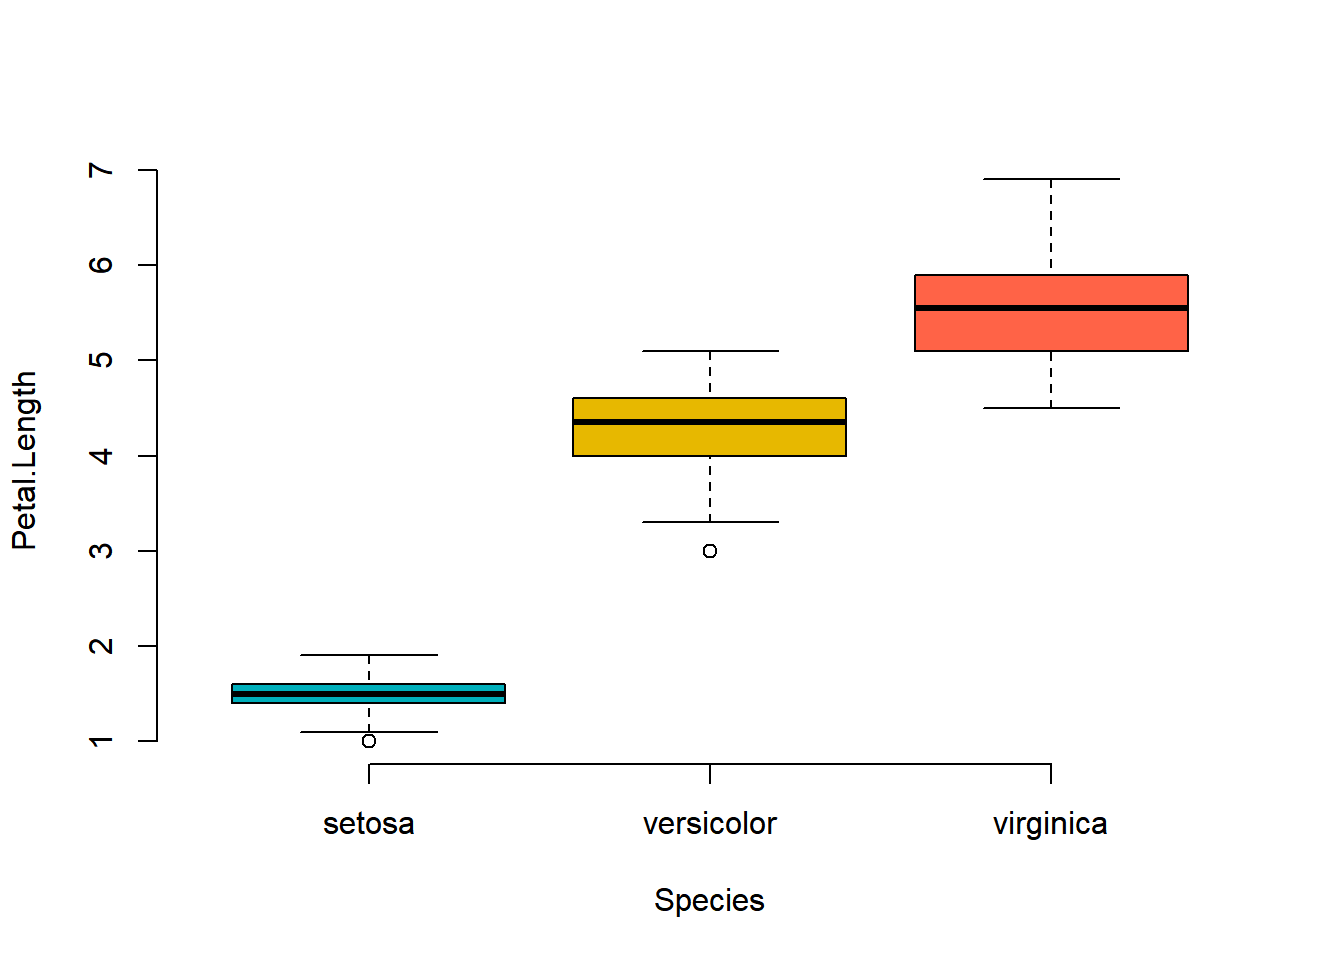
\includegraphics{ANOVA-Multi_files/figure-latex/unnamed-chunk-2-2.pdf}

boxplot으로 나타내면 위와 같이 구성되어 있다.

종속변수에 길이에 대한 변수만 다루겠다.

\hypertarget{manova}{%
\subsection{MANOVA}\label{manova}}

귀무가설 : 모든 평균들은 다 같다.

대체가설 : 평균들이 모두 같지는 않다. ('평균들이 모두 다르다'가 아니다.)

\hypertarget{manova-test}{%
\section{MANOVA test}\label{manova-test}}

sepl \textless- iris\(Sepal.Length petl <- iris\)Petal.Length

\begin{Shaded}
\begin{Highlighting}[]
\NormalTok{res.man }\OtherTok{\textless{}{-}} \FunctionTok{manova}\NormalTok{(}\FunctionTok{cbind}\NormalTok{(Sepal.Length, Petal.Length) }\SpecialCharTok{\textasciitilde{}}\NormalTok{ Species, }\AttributeTok{data =}\NormalTok{ iris)}

\FunctionTok{summary}\NormalTok{(res.man)}
\end{Highlighting}
\end{Shaded}

\begin{verbatim}
##            Df Pillai approx F num Df den Df    Pr(>F)    
## Species     2 0.9885   71.829      4    294 < 2.2e-16 ***
## Residuals 147                                            
## ---
## Signif. codes:  0 '***' 0.001 '**' 0.01 '*' 0.05 '.' 0.1 ' ' 1
\end{verbatim}

p값이 유의수준보다 작기 때문에 통계적으로 유의하다.

즉, 분꽃의 종에 따라 꽃받침 길이, 꽃잎의 길이 차가 있다.

\begin{Shaded}
\begin{Highlighting}[]
\FunctionTok{summary.aov}\NormalTok{(res.man)}
\end{Highlighting}
\end{Shaded}

\begin{verbatim}
##  Response Sepal.Length :
##              Df Sum Sq Mean Sq F value    Pr(>F)    
## Species       2 63.212  31.606  119.26 < 2.2e-16 ***
## Residuals   147 38.956   0.265                      
## ---
## Signif. codes:  0 '***' 0.001 '**' 0.01 '*' 0.05 '.' 0.1 ' ' 1
## 
##  Response Petal.Length :
##              Df Sum Sq Mean Sq F value    Pr(>F)    
## Species       2 437.10 218.551  1180.2 < 2.2e-16 ***
## Residuals   147  27.22   0.185                      
## ---
## Signif. codes:  0 '***' 0.001 '**' 0.01 '*' 0.05 '.' 0.1 ' ' 1
\end{verbatim}

종속변수의 변수 각각을 보고싶다면 summary.aov 함수를 사용한다.

\hypertarget{uxd68cuxadc0uxbaa8uxd615regression-model}{%
\section{회귀모형(Regression Model)}\label{uxd68cuxadc0uxbaa8uxd615regression-model}}

\hypertarget{uxb370uxc774uxd130-uxbd88uxb7ecuxc624uxae30-6}{%
\subsection{데이터 불러오기}\label{uxb370uxc774uxd130-uxbd88uxb7ecuxc624uxae30-6}}

\begin{Shaded}
\begin{Highlighting}[]
\FunctionTok{data}\NormalTok{(women)}
\FunctionTok{str}\NormalTok{(women)}
\end{Highlighting}
\end{Shaded}

\begin{verbatim}
## 'data.frame':    15 obs. of  2 variables:
##  $ height: num  58 59 60 61 62 63 64 65 66 67 ...
##  $ weight: num  115 117 120 123 126 129 132 135 139 142 ...
\end{verbatim}

women(여성 데이터셋)
-height: 키(단위:in)
-weight: 몸무게(단위:lb)

R에 있는 기본 데이터셋인 women을 불러온다.

2개의 변수와 15개의 관측치가 있다.

\hypertarget{uxc0c1uxad00-uxbd84uxc11d}{%
\subsection{상관 분석}\label{uxc0c1uxad00-uxbd84uxc11d}}

여성의 키와 몸무게의 인과관계를 위한 회귀분석하기 전에,

두 변수의 상관성을 알아본다.

\begin{Shaded}
\begin{Highlighting}[]
\FunctionTok{cor}\NormalTok{(women}\SpecialCharTok{$}\NormalTok{height,women}\SpecialCharTok{$}\NormalTok{weight)}
\end{Highlighting}
\end{Shaded}

\begin{verbatim}
## [1] 0.9954948
\end{verbatim}

\begin{Shaded}
\begin{Highlighting}[]
\FunctionTok{cor.test}\NormalTok{(women}\SpecialCharTok{$}\NormalTok{height,women}\SpecialCharTok{$}\NormalTok{weight)}
\end{Highlighting}
\end{Shaded}

\begin{verbatim}
## 
##  Pearson's product-moment correlation
## 
## data:  women$height and women$weight
## t = 37.855, df = 13, p-value = 1.091e-14
## alternative hypothesis: true correlation is not equal to 0
## 95 percent confidence interval:
##  0.9860970 0.9985447
## sample estimates:
##       cor 
## 0.9954948
\end{verbatim}

상관계수가 1에 가까울수록 두 변수의 상관력이 높다는 의미다.

0.99로 아주 높다.

\#\#회귀모형 찾기

\hypertarget{uxd68cuxadc0uxbaa8uxd615}{%
\subsubsection{회귀모형}\label{uxd68cuxadc0uxbaa8uxd615}}

\begin{Shaded}
\begin{Highlighting}[]
\NormalTok{fit1 }\OtherTok{\textless{}{-}} \FunctionTok{lm}\NormalTok{(weight}\SpecialCharTok{\textasciitilde{}}\NormalTok{height, }\AttributeTok{data =}\NormalTok{ women)}
\FunctionTok{summary}\NormalTok{(fit1)}
\end{Highlighting}
\end{Shaded}

\begin{verbatim}
## 
## Call:
## lm(formula = weight ~ height, data = women)
## 
## Residuals:
##     Min      1Q  Median      3Q     Max 
## -1.7333 -1.1333 -0.3833  0.7417  3.1167 
## 
## Coefficients:
##              Estimate Std. Error t value Pr(>|t|)    
## (Intercept) -87.51667    5.93694  -14.74 1.71e-09 ***
## height        3.45000    0.09114   37.85 1.09e-14 ***
## ---
## Signif. codes:  0 '***' 0.001 '**' 0.01 '*' 0.05 '.' 0.1 ' ' 1
## 
## Residual standard error: 1.525 on 13 degrees of freedom
## Multiple R-squared:  0.991,  Adjusted R-squared:  0.9903 
## F-statistic:  1433 on 1 and 13 DF,  p-value: 1.091e-14
\end{verbatim}

\begin{itemize}
\tightlist
\item
  Call: 사용한 식
\item
  Residusals(잔차): 실제값과 오차
\item
  귀무가설: 회귀계수가 0이다.
\item
  R-squared(결정 계수): 설명력 : 99.1\% 만큼 실제값의 산포도와 일치한다.(실제 분산의 얼마만큼 잘 설명하는가)
\item
  결정 계수는 주어진 종속변수(표본)과 추정한 종속변수 간의 상관계수의 제곱이다.
\item
  F-statistic: 귀무가설: 두 변수는 선형관계가 없다.
\end{itemize}

선형 회귀 모형의 결과, 절편과 height 통계적으로 둘 다 고도로 유의한 결과가 나왔다.

그리고 R-squared 값이 0.991로 아주 높은 값이 나와 적합한 모형이라 볼 수 있다.

모형의 결과는,

weight = -87.51667 + 3.45 x height

\hypertarget{plot}{%
\subsubsection{plot}\label{plot}}

\begin{Shaded}
\begin{Highlighting}[]
\FunctionTok{plot}\NormalTok{(}\AttributeTok{x =}\NormalTok{ women}\SpecialCharTok{$}\NormalTok{height, }\AttributeTok{y =}\NormalTok{ women}\SpecialCharTok{$}\NormalTok{weight, }
     \AttributeTok{xlab =} \StringTok{\textquotesingle{}Height (inches)\textquotesingle{}}\NormalTok{, }\AttributeTok{ylab =} \StringTok{\textquotesingle{}Weight (lbs)\textquotesingle{}}\NormalTok{)}
\FunctionTok{abline}\NormalTok{(fit1)}
\end{Highlighting}
\end{Shaded}

\includegraphics{RegressionModel_files/figure-latex/unnamed-chunk-5-1.pdf}

실제 데이터 그래프에 회귀방정식을 그려보면,

거의 일치한 모습을 볼 수 있다.

좀 더 자세한 그래프를 그려보자.

\hypertarget{scatterplot}{%
\subsubsection{scatterplot}\label{scatterplot}}

\begin{Shaded}
\begin{Highlighting}[]
\FunctionTok{library}\NormalTok{(car)}
\end{Highlighting}
\end{Shaded}

\begin{verbatim}
## Loading required package: carData
\end{verbatim}

\begin{Shaded}
\begin{Highlighting}[]
\FunctionTok{scatterplot}\NormalTok{(}
\NormalTok{  weight }\SpecialCharTok{\textasciitilde{}}\NormalTok{ height, }
  \AttributeTok{data =}\NormalTok{ women, }
  \AttributeTok{spread =} \ConstantTok{FALSE}\NormalTok{, }
  \AttributeTok{smoother.args =} \FunctionTok{list}\NormalTok{(}\AttributeTok{lty=}\DecValTok{2}\NormalTok{), }
  \AttributeTok{pch =} \DecValTok{19}\NormalTok{,}
  \AttributeTok{main =} \StringTok{\textquotesingle{}Women Age 30 \textasciitilde{} 39\textquotesingle{}}\NormalTok{,}
  \AttributeTok{xlab =} \StringTok{\textquotesingle{}Height (inches)\textquotesingle{}}\NormalTok{,}
  \AttributeTok{ylab =} \StringTok{\textquotesingle{}Weight (lbs)\textquotesingle{}} 
\NormalTok{)}
\end{Highlighting}
\end{Shaded}

\begin{verbatim}
## Warning in plot.window(...): "spread" is not a graphical parameter
\end{verbatim}

\begin{verbatim}
## Warning in plot.window(...): "smoother.args" is not a graphical parameter
\end{verbatim}

\begin{verbatim}
## Warning in plot.xy(xy, type, ...): "spread" is not a graphical parameter
\end{verbatim}

\begin{verbatim}
## Warning in plot.xy(xy, type, ...): "smoother.args" is not a graphical parameter
\end{verbatim}

\begin{verbatim}
## Warning in axis(side = side, at = at, labels = labels, ...): "spread" is not a
## graphical parameter
\end{verbatim}

\begin{verbatim}
## Warning in axis(side = side, at = at, labels = labels, ...): "smoother.args" is
## not a graphical parameter
\end{verbatim}

\begin{verbatim}
## Warning in axis(side = side, at = at, labels = labels, ...): "spread" is not a
## graphical parameter
\end{verbatim}

\begin{verbatim}
## Warning in axis(side = side, at = at, labels = labels, ...): "smoother.args" is
## not a graphical parameter
\end{verbatim}

\begin{verbatim}
## Warning in box(...): "spread" is not a graphical parameter
\end{verbatim}

\begin{verbatim}
## Warning in box(...): "smoother.args" is not a graphical parameter
\end{verbatim}

\begin{verbatim}
## Warning in title(...): "spread" is not a graphical parameter
\end{verbatim}

\begin{verbatim}
## Warning in title(...): "smoother.args" is not a graphical parameter
\end{verbatim}

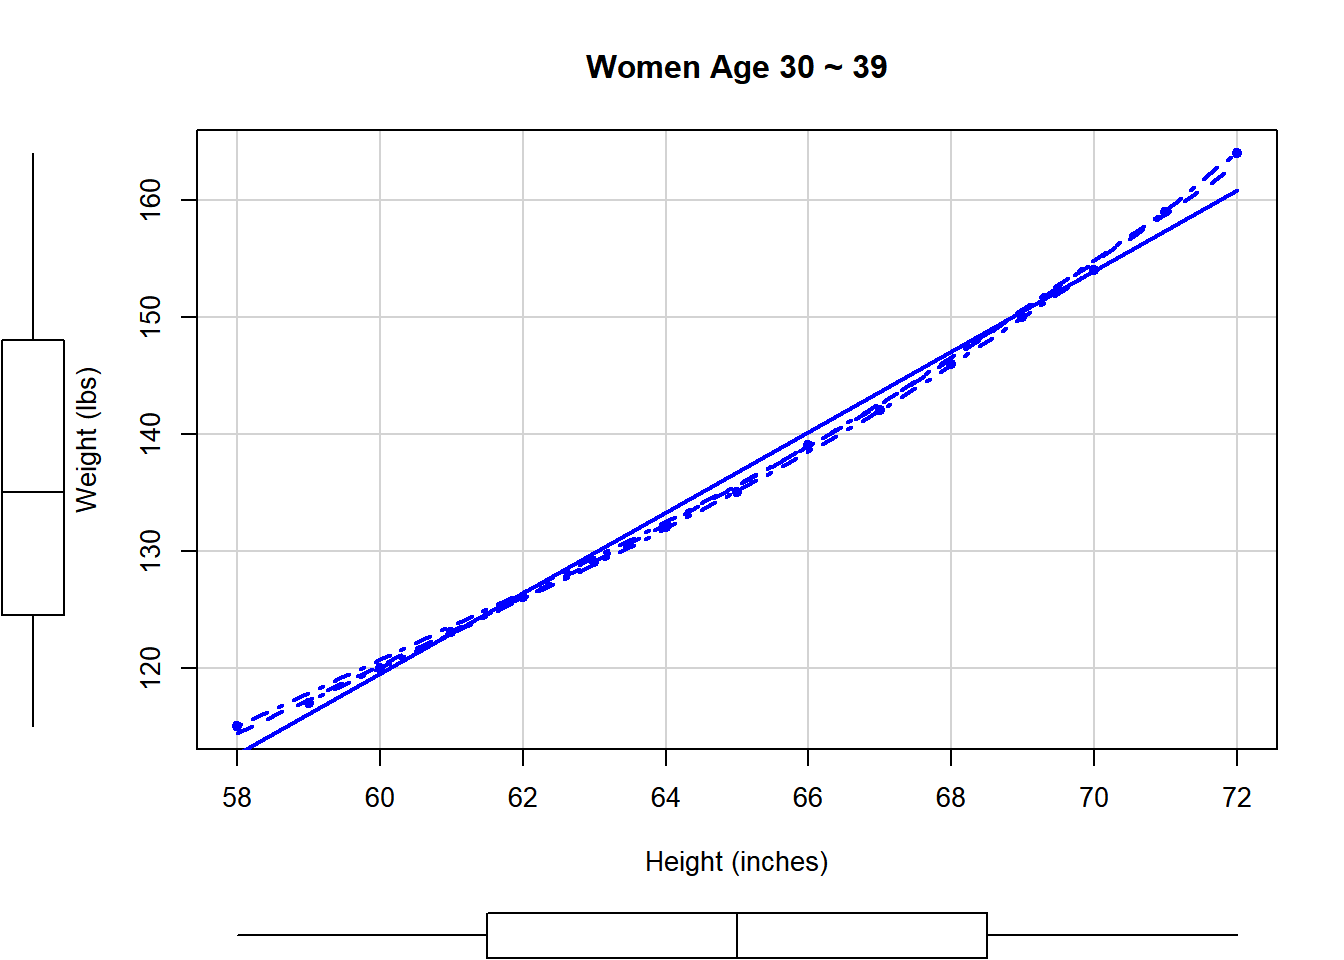
\includegraphics{RegressionModel_files/figure-latex/unnamed-chunk-6-1.pdf}

\begin{Shaded}
\begin{Highlighting}[]
\CommentTok{\#lty는 ling type}
\CommentTok{\#회귀분석후 그래프까지 나타내줌}
\CommentTok{\#회귀분석 결과를 선으로 나타난다.(평활선(loess)(smoother):모난부분을 부드럽게 해준다.)}
\CommentTok{\#직선보다 더 좋게 만들 수 있다.(회귀모형에 대한 힌트를 준다.)}
\end{Highlighting}
\end{Shaded}

\hypertarget{uxb2e4uxd56duxd68cuxadc0uxbaa8uxd615}{%
\subsection{다항회귀모형}\label{uxb2e4uxd56duxd68cuxadc0uxbaa8uxd615}}

독립변수의 차수가 2차 이상인 회귀모형이다.

\begin{Shaded}
\begin{Highlighting}[]
\NormalTok{fit2 }\OtherTok{\textless{}{-}} \FunctionTok{lm}\NormalTok{(weight}\SpecialCharTok{\textasciitilde{}}\NormalTok{height}\SpecialCharTok{+}\FunctionTok{I}\NormalTok{(height}\SpecialCharTok{\^{}}\DecValTok{2}\NormalTok{), }\AttributeTok{data =}\NormalTok{ women)}
\FunctionTok{summary}\NormalTok{(fit2)}
\end{Highlighting}
\end{Shaded}

\begin{verbatim}
## 
## Call:
## lm(formula = weight ~ height + I(height^2), data = women)
## 
## Residuals:
##      Min       1Q   Median       3Q      Max 
## -0.50941 -0.29611 -0.00941  0.28615  0.59706 
## 
## Coefficients:
##              Estimate Std. Error t value Pr(>|t|)    
## (Intercept) 261.87818   25.19677  10.393 2.36e-07 ***
## height       -7.34832    0.77769  -9.449 6.58e-07 ***
## I(height^2)   0.08306    0.00598  13.891 9.32e-09 ***
## ---
## Signif. codes:  0 '***' 0.001 '**' 0.01 '*' 0.05 '.' 0.1 ' ' 1
## 
## Residual standard error: 0.3841 on 12 degrees of freedom
## Multiple R-squared:  0.9995, Adjusted R-squared:  0.9994 
## F-statistic: 1.139e+04 on 2 and 12 DF,  p-value: < 2.2e-16
\end{verbatim}

fit1과 마찬가지로 적합한 회귀모형이다.

R-squared가 조금 더 높은 것으로 보아

더 많은 데이터를 설명해줄 수 있는 모형이다.

모형의 결과는,

\textbf{weight = 261.87818 - 7.34832 x height + 0.08306 x height\^{}2}

\begin{Shaded}
\begin{Highlighting}[]
\FunctionTok{with}\NormalTok{(}\AttributeTok{data =}\NormalTok{ women, }\AttributeTok{expr =}\NormalTok{ \{}
  \FunctionTok{plot}\NormalTok{(}\AttributeTok{x =}\NormalTok{ height, }\AttributeTok{y =}\NormalTok{ weight, }\AttributeTok{xlab =} \StringTok{\textquotesingle{}Height (inches)\textquotesingle{}}\NormalTok{, }\AttributeTok{ylab =} \StringTok{\textquotesingle{}Weight (lbs)\textquotesingle{}}\NormalTok{)}
  \FunctionTok{lines}\NormalTok{(}\AttributeTok{x =}\NormalTok{ height, }\AttributeTok{y =} \FunctionTok{fitted}\NormalTok{(fit2))}
\NormalTok{\})}
\end{Highlighting}
\end{Shaded}

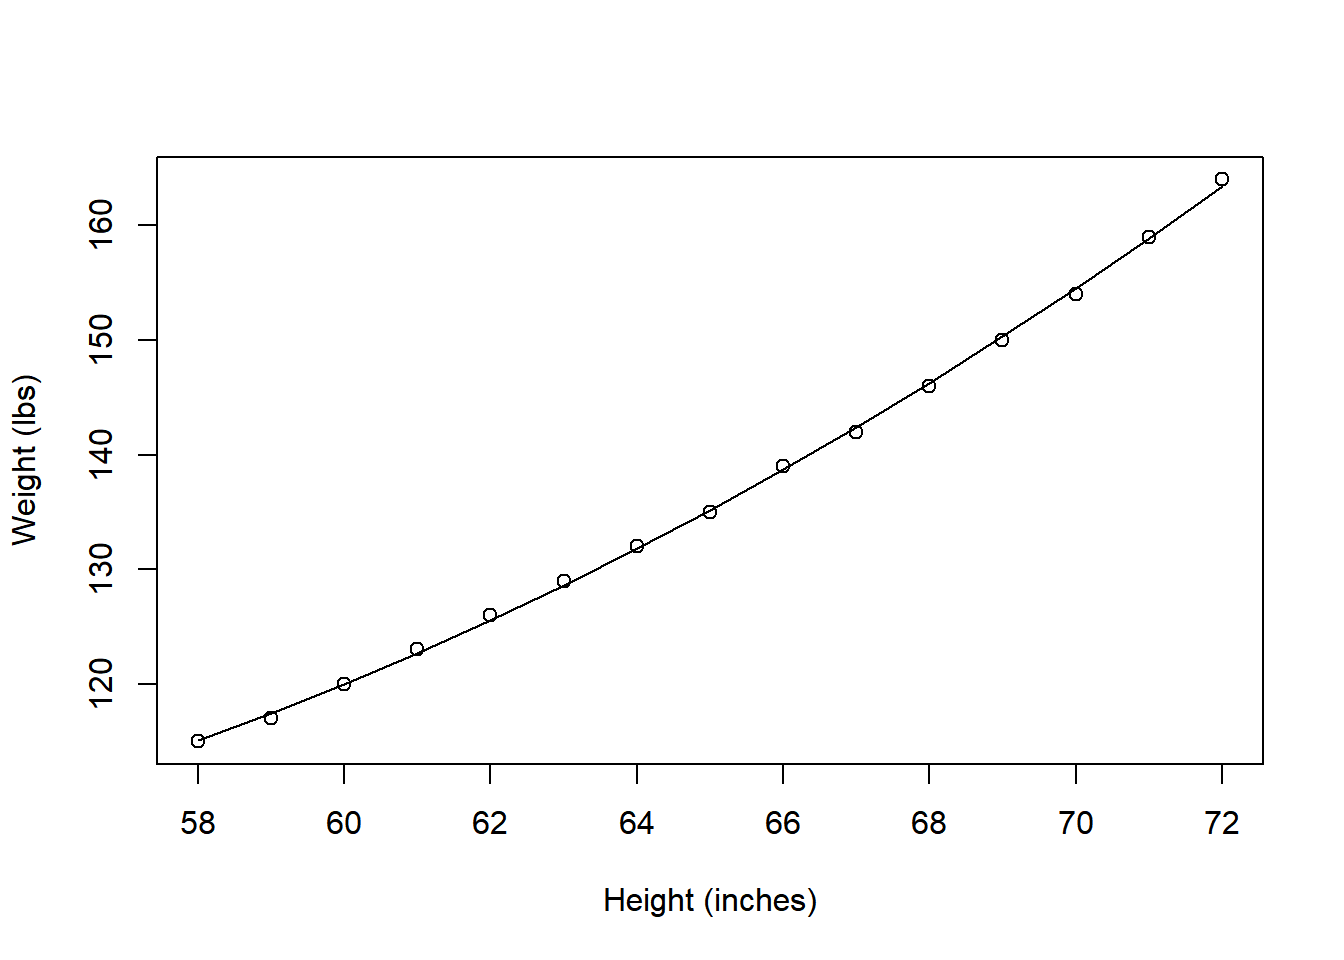
\includegraphics{RegressionModel_files/figure-latex/unnamed-chunk-9-1.pdf}

그래프로 보았을때, 확실히 fit1보다 더 많은 데이터에 적합하다.

\end{document}
